% \documentclass[11pt, a4paper, twoside]{article} % Usar para imprimir
\documentclass[10pt, a4paper]{article}

%%%%%%%%%%%%%%%%%%%%%%%%%%%%%%%%%%%%%%%%%%%%%%%%%%%%%%%%%%%%%%%%%%%%%%%%%%
%
% Plantilla para libro de texto de matemáticas.
%
% Esta plantilla ha sido desarrollada desde cero, pero utiliza algunas partes
% del código de la plantilla original utilizada en apuntesDGIIM
% (https://github.com/libreim/apuntesDGIIM), basada a su vez en las plantillas
% 'Short Sectioned Assignment' de Frits Wenneker (http://www.howtotex.com),
% 'Plantilla de Trabajo' de Mario Román y 'Plantilla básica de Latex en Español'
% de Andrés Herrera Poyatos (https://github.com/andreshp). También recoge
% ideas de la plantilla 'Multi-Purpose Large Font Title Page' de
% Frits Wenneker y Vel (vel@latextemplates.com).
%
% Licencia:
% CC BY-NC-SA 4.0 (https://creativecommons.org/licenses/by-nc-sa/4.0/)
%
%%%%%%%%%%%%%%%%%%%%%%%%%%%%%%%%%%%%%%%%%%%%%%%%%%%%%%%%%%%%%%%%%%%%%%%%%

% ---------------------------------------------------------------------------
% CONFIGURACIÓN BÁSICA DEL DOCUMENTO
% ---------------------------------------------------------------------------

\usepackage[hyphens]{url}
\linespread{1.3}            % Espaciado entre líneas.
\setlength\parindent{0pt}   % No indentar el texto por defecto.
\setlength\parskip{7pt}

\usepackage{multirow}
\usepackage{xcolor,colortbl}
\usepackage{fancyvrb,newverbs,xcolor}
\usepackage{lipsum} % just for this example

\definecolor{cverbbg}{gray}{0.93}

\newenvironment{cverbatim}
 {\SaveVerbatim{cverb}}
 {\endSaveVerbatim
  \flushleft\fboxrule=0pt\fboxsep=.5em
  \colorbox{cverbbg}{\BUseVerbatim{cverb}}%
  \endflushleft
}
\newenvironment{lcverbatim}
 {\SaveVerbatim{cverb}}
 {\endSaveVerbatim
  \flushleft\fboxrule=0pt\fboxsep=.5em
  \colorbox{cverbbg}{%
    \makebox[\dimexpr\linewidth-2\fboxsep][l]{\BUseVerbatim{cverb}}%
  }
  \endflushleft
}

\newcommand{\ctexttt}[1]{\colorbox{cverbbg}{\texttt{#1}}}
\newverbcommand{\cverb}
  {\setbox\verbbox\hbox\bgroup}
  {\egroup\colorbox{cverbbg}{\box\verbbox}}

\usepackage[normalem]{ulem}
\usepackage{cancel}
\newcommand\dout{\bgroup \markoverwith{\rule[0.2ex]{0.1pt}{0.4pt}\rule[0.8ex]{0.1pt}{0.4pt}}\ULon}
\def\dout{\bgroup
 \markoverwith{\lower-0.35ex\hbox
 {\kern-.03em\vbox{\hrule width.2em\kern0.45ex\hrule}\kern-.03em}}%
 \ULon}
\MakeRobust\dout


% ---------------------------------------------------------------------------
% PAQUETES BÁSICOS
% ---------------------------------------------------------------------------

% IDIOMA
\usepackage[utf8]{inputenc}
\usepackage[spanish, es-tabla, es-lcroman, es-noquoting]{babel}

% MATEMÁTICAS
\usepackage{amsmath}    % Paquete básico de matemáticas
\usepackage{amsthm}     % Teoremas
\usepackage{mathrsfs}   % Fuente para ciertas letras utilizadas en matemáticas

% FUENTES
\usepackage{newpxtext, newpxmath}   % Fuente similar a Palatino
\usepackage{FiraSans}                 % Fuente sans serif
\usepackage[T1]{fontenc}
\usepackage[italic]{mathastext}     % Utiliza la fuente del documento
                                    % en los entornos matemáticos

% MÁRGENES
\usepackage[margin=2.5cm, top=3cm]{geometry}

% LISTAS
\usepackage{enumitem}       % Mejores listas
\setlist{leftmargin=.5in}   % Especifica la indentación para las listas.

% Listas ordenadas con números romanos (i), (ii), etc.
\newenvironment{nlist}
{\begin{enumerate}
    \renewcommand\labelenumi{(\emph{\roman{enumi})}}}
  {\end{enumerate}}

%  OTROS
\usepackage[hidelinks]{hyperref}   % Enlaces
\usepackage{graphicx}   % Permite incluir gráficos en el documento
\usepackage{relsize}

% LISTINGS
\usepackage{listings}
\usepackage{xcolor}     % Permite definir y utilizar colores
\usepackage{lipsum}
\usepackage{courier}

% Fijar tabla a posición
\usepackage{array}
\newcolumntype{L}[1]{>{\raggedright\let\newline\\\arraybackslash\hspace{0pt}}m{#1}}
\newcolumntype{C}[1]{>{\centering\let\newline\\\arraybackslash\hspace{0pt}}m{#1}}
\newcolumntype{R}[1]{>{\raggedleft\let\newline\\\arraybackslash\hspace{0pt}}m{#1}}

% Colores para los bloques de código
\definecolor{codegreen}{rgb}{0,0.6,0}
\definecolor{codegray}{rgb}{0.5,0.5,0.5}
\definecolor{codepurple}{rgb}{0.58,0,0.82}
\definecolor{backcolour}{rgb}{0.95,0.95,0.92}
\lstdefinestyle{mystyle}{
	backgroundcolor=\color{backcolour},   
	commentstyle=\color{codegreen},
	keywordstyle=\color{blue},
	numberstyle=\tiny\color{codegray},
	stringstyle=\color{codepurple},
	basicstyle=\footnotesize\ttfamily,
	breakatwhitespace=false,         
	breaklines=true,                 
	captionpos=b,                    
	keepspaces=true,                 
	numbers=left,                    
	numbersep=5pt,                  
	showspaces=false,                
	showstringspaces=false,
	showtabs=false,                  
	tabsize=4
}
\lstset{style=mystyle}

%\lstset{basicstyle=\footnotesize\ttfamily,breaklines=true}
%\lstset{framextopmargin=50pt,frame=bottomline}
 
% ---------------------------------------------------------------------------
% COMANDOS PERSONALIZADOS
% ---------------------------------------------------------------------------

% \equalto
\newcommand{\verteq}{\rotatebox{90}{$\,=$}}
\newcommand{\equalto}[2]{\underset{\scriptstyle\overset{\mkern4mu\verteq}{#2}}{#1}}

% ---------------------------------------------------------------------------
% COLORES
% ---------------------------------------------------------------------------

\definecolor{50}{HTML}{fbe9e7}
\definecolor{100}{HTML}{ffccbc}
\definecolor{200}{HTML}{ffab91}
\definecolor{300}{HTML}{ff8a65}
\definecolor{400}{HTML}{ff7043}
\definecolor{500}{HTML}{ff5722}
\definecolor{600}{HTML}{f4511e}
\definecolor{700}{HTML}{e64a19}
\definecolor{800}{HTML}{d84315}
\definecolor{900}{HTML}{bf360c}

% ---------------------------------------------------------------------------
% DISEÑO DE PÁGINA
% ---------------------------------------------------------------------------

\usepackage{pagecolor}
\usepackage{afterpage}

% ---------------------------------------------------------------------------
% CABECERA Y PIE DE PÁGINA
% ---------------------------------------------------------------------------

\usepackage{fancyhdr}   % Paquete para cabeceras y pies de página

% Indica que las páginas usarán la configuración de fancyhdr
\pagestyle{fancy}
\fancyhf{}

% Representa la sección de la cabecera
\renewcommand{\sectionmark}[1]{%
\markboth{#1}{}}

% Representa la subsección de la cabecera
\renewcommand{\sectionmark}[1]{%
\markright{#1}{}}

% Parte derecha de la cabecera
\fancyhead[LE,RO]{\sffamily\textsl{Práctica 3: Modelo Jerárquico} \hspace{1em}  \textcolor{500}{\rule[-0.4ex]{0.2ex}{1.2em}} \hspace{1em} \thepage}

\let\Oldpart\part
\newcommand{\parttitle}{}
\renewcommand{\part}[1]{\pagebreak\Oldpart{#1}\renewcommand{\parttitle}{#1}}

% Parte izquierda de la cabecera
\fancyhead[RE,LO]{\sffamily{\parttitle}}

% Elimina la línea de la cabecera
\renewcommand{\headrulewidth}{0pt}

% Controla la altura de la cabecera para que no haya errores
\setlength{\headheight}{14pt}

% ---------------------------------------------------------------------------
% TÍTULOS DE PARTES Y SECCIONES
% ---------------------------------------------------------------------------

\usepackage{titlesec}

% Estilo de los títulos de las partes
\titleformat{\part}[hang]{\Huge\bfseries\sffamily}{\thepart\hspace{20pt}\textcolor{500}{|}\hspace{20pt}}{0pt}{\Huge\bfseries}
\titlespacing*{\part}{0cm}{-2em}{2em}[0pt]

% Reiniciamos el contador de secciones entre partes (opcional)
\makeatletter
\@addtoreset{section}{part}
\makeatother

% Estilo de los títulos de las secciones, subsecciones y subsubsecciones
\titleformat{\section}
  {\Large\bfseries\sffamily}{\thesection}{1em}{}

\titleformat{\subsection}
  {\Large\sffamily}{\thesubsection}{1em}{}[\vspace{.5em}]

\titleformat{\subsubsection}
  {\sffamily}{\thesubsubsection}{1em}{}

% ---------------------------------------------------------------------------
% ENTORNOS PERSONALIZADOS
% ---------------------------------------------------------------------------

\usepackage{mdframed}

%% DEFINICIONES DE LOS ESTILOS

% Nuevo estilo para definiciones
\newtheoremstyle{definition-style}  % Nombre del estilo
{}                                  % Espacio por encima
{}                                  % Espacio por debajo
{}                                  % Fuente del cuerpo
{}                                  % Identación
{\bf\sffamily}                      % Fuente para la cabecera
{.}                                 % Puntuación tras la cabecera
{.5em}                              % Espacio tras la cabecera
{\thmname{#1}\thmnumber{ #2}\thmnote{ (#3)}}  % Especificación de la cabecera

% Nuevo estilo para notas
\newtheoremstyle{remark-style}
{10pt}
{10pt}
{}
{}
{\itshape \sffamily}
{.}
{.5em}
{}

% Nuevo estilo para teoremas y proposiciones
\newtheoremstyle{theorem-style}
{}
{}
{}
{}
{\bfseries \sffamily}
{.}
{.5em}
{\thmname{#1}\thmnumber{ #2}\thmnote{ (#3)}}

% Nuevo estilo para ejemplos
\newtheoremstyle{example-style}
{10pt}
{10pt}
{}
{}
{\bf \sffamily}
{}
{.5em}
{\thmname{#1}\thmnumber{ #2.}\thmnote{ #3.}}

% Nuevo estilo para la demostración

\makeatletter
\renewenvironment{proof}[1][\proofname] {\par\pushQED{\qed}\normalfont\topsep6\p@\@plus6\p@\relax\trivlist\item[\hskip\labelsep\itshape\sffamily#1\@addpunct{.}]\ignorespaces}{\popQED\endtrivlist\@endpefalse}
\makeatother

%% ASIGNACIÓN DE LOS ESTILOS

% Teoremas, proposiciones y corolarios
\newtheoremstyle{theorem-style}{}{}{}{}{}{}{ }{}
\theoremstyle{theorem-style}
\newtheorem*{datos}{}
\theoremstyle{theorem-style}
\newtheorem{nth}{Teorema}[section]
\newtheorem{nprop}{Proposición}[section]
\newtheorem{ncor}{Corolario}[section]
\newtheorem{lema}{Lema}[section]

% Definiciones
\theoremstyle{definition-style}
\newtheorem{ndef}{Definición}[section]

% Notas
\theoremstyle{remark-style}
\newtheorem*{nota}{Nota}

% Ejemplos
\theoremstyle{example-style}
\newtheorem{ejemplo}{Ejemplo}[section]

% Ejercicios y solución
\theoremstyle{definition-style}
\newtheorem{ejer}{Ejercicio}[section]

\theoremstyle{remark-style}
\newtheorem*{sol}{Solución}

%% MARCOS DE LOS ESTILOS

% Configuración general de mdframe, los estilos de los teoremas, etc
\mdfsetup{
  skipabove=1em,
  skipbelow=1em,
  innertopmargin=1em,
  innerbottommargin=1em,
  splittopskip=2\topsep,
}

% Definimos los marcos de los estilos
\mdfdefinestyle{datos-frame}{
	linewidth=2pt, %
	linecolor= 500, %
	topline=false, %
	bottomline=false, %
	rightline=false,%
	leftmargin=0em, %
	innerleftmargin=1em, %
	innerrightmargin=1em,
	rightmargin=0em, %
}%
\mdfdefinestyle{nth-frame}{
	linewidth=2pt, %
	linecolor= 500, %
	topline=false, %
	bottomline=false, %
	rightline=false,%
	leftmargin=0em, %
	innerleftmargin=1em, %
  innerrightmargin=1em,
	rightmargin=0em, %
}%

\mdfdefinestyle{nprop-frame}{
	linewidth=2pt, %
	linecolor= 300, %
	topline=false, %
	bottomline=false, %
	rightline=false,%
	leftmargin=0pt, %
	innerleftmargin=1em, %
	innerrightmargin=1em,
	rightmargin=0pt, %
}%

\mdfdefinestyle{ndef-frame}{
	linewidth=2pt, %
	linecolor= 500, %
	backgroundcolor= 50,
	topline=false, %
	bottomline=false, %
	rightline=false,%
	leftmargin=0pt, %
	innerleftmargin=1em, %
	innerrightmargin=1em,
	rightmargin=0pt, %
}%

\mdfdefinestyle{ejer-frame}{
	linewidth=2pt, %
	linecolor= 300, %
	backgroundcolor= 50,
	topline=false, %
	bottomline=false, %
	rightline=false,%
	leftmargin=0pt, %
	innerleftmargin=1em, %
	innerrightmargin=1em,
	rightmargin=0pt, %
}%

\mdfdefinestyle{ejemplo-frame}{
	linewidth=0pt, %
	linecolor= 300, %
	leftline=false, %
	rightline=false, %
	leftmargin=0pt, %
	innerleftmargin=1.3em, %
	innerrightmargin=1em,
	rightmargin=0pt, %
	innertopmargin=0em,%
	innerbottommargin=0em, %
	splittopskip=\topskip, %
}%

% Asignamos los marcos a los estilos
\surroundwithmdframed[style=nth-frame]{nth}
\surroundwithmdframed[style=datos-frame]{datos}
\surroundwithmdframed[style=nprop-frame]{nprop}
\surroundwithmdframed[style=nprop-frame]{ncor}
\surroundwithmdframed[style=ndef-frame]{ndef}
\surroundwithmdframed[style=ejer-frame]{ejer}
\surroundwithmdframed[style=ejemplo-frame]{ejemplo}
\surroundwithmdframed[style=ejemplo-frame]{sol}

%---------------------------------------
% BlackBoard Math Fonts :-
%---------------------------------------

%Captital Letters
\newcommand{\bbA}{\mathbb{A}}	\newcommand{\bbB}{\mathbb{B}}
\newcommand{\bbC}{\mathbb{C}}	\newcommand{\bbD}{\mathbb{D}}
\newcommand{\bbE}{\mathbb{E}}	\newcommand{\bbF}{\mathbb{F}}
\newcommand{\bbG}{\mathbb{G}}	\newcommand{\bbH}{\mathbb{H}}
\newcommand{\bbI}{\mathbb{I}}	\newcommand{\bbJ}{\mathbb{J}}
\newcommand{\bbK}{\mathbb{K}}	\newcommand{\bbL}{\mathbb{L}}
\newcommand{\bbM}{\mathbb{M}}	\newcommand{\bbN}{\mathbb{N}}
\newcommand{\bbO}{\mathbb{O}}	\newcommand{\bbP}{\mathbb{P}}
\newcommand{\bbQ}{\mathbb{Q}}	\newcommand{\bbR}{\mathbb{R}}
\newcommand{\bbS}{\mathbb{S}}	\newcommand{\bbT}{\mathbb{T}}
\newcommand{\bbU}{\mathbb{U}}	\newcommand{\bbV}{\mathbb{V}}
\newcommand{\bbW}{\mathbb{W}}	\newcommand{\bbX}{\mathbb{X}}
\newcommand{\bbY}{\mathbb{Y}}	\newcommand{\bbZ}{\mathbb{Z}}

%---------------------------------------
% MathCal Fonts :-
%---------------------------------------

%Captital Letters
\newcommand{\mcA}{\mathcal{A}}	\newcommand{\mcB}{\mathcal{B}}
\newcommand{\mcC}{\mathcal{C}}	\newcommand{\mcD}{\mathcal{D}}
\newcommand{\mcE}{\mathcal{E}}	\newcommand{\mcF}{\mathcal{F}}
\newcommand{\mcG}{\mathcal{G}}	\newcommand{\mcH}{\mathcal{H}}
\newcommand{\mcI}{\mathcal{I}}	\newcommand{\mcJ}{\mathcal{J}}
\newcommand{\mcK}{\mathcal{K}}	\newcommand{\mcL}{\mathcal{L}}
\newcommand{\mcM}{\mathcal{M}}	\newcommand{\mcN}{\mathcal{N}}
\newcommand{\mcO}{\mathcal{O}}	\newcommand{\mcP}{\mathcal{P}}
\newcommand{\mcQ}{\mathcal{Q}}	\newcommand{\mcR}{\mathcal{R}}
\newcommand{\mcS}{\mathcal{S}}	\newcommand{\mcT}{\mathcal{T}}
\newcommand{\mcU}{\mathcal{U}}	\newcommand{\mcV}{\mathcal{V}}
\newcommand{\mcW}{\mathcal{W}}	\newcommand{\mcX}{\mathcal{X}}
\newcommand{\mcY}{\mathcal{Y}}	\newcommand{\mcZ}{\mathcal{Z}}


%---------------------------------------
% Bold Math Fonts :-
%---------------------------------------

%Captital Letters
\newcommand{\bmA}{\boldsymbol{A}}	\newcommand{\bmB}{\boldsymbol{B}}
\newcommand{\bmC}{\boldsymbol{C}}	\newcommand{\bmD}{\boldsymbol{D}}
\newcommand{\bmE}{\boldsymbol{E}}	\newcommand{\bmF}{\boldsymbol{F}}
\newcommand{\bmG}{\boldsymbol{G}}	\newcommand{\bmH}{\boldsymbol{H}}
\newcommand{\bmI}{\boldsymbol{I}}	\newcommand{\bmJ}{\boldsymbol{J}}
\newcommand{\bmK}{\boldsymbol{K}}	\newcommand{\bmL}{\boldsymbol{L}}
\newcommand{\bmM}{\boldsymbol{M}}	\newcommand{\bmN}{\boldsymbol{N}}
\newcommand{\bmO}{\boldsymbol{O}}	\newcommand{\bmP}{\boldsymbol{P}}
\newcommand{\bmQ}{\boldsymbol{Q}}	\newcommand{\bmR}{\boldsymbol{R}}
\newcommand{\bmS}{\boldsymbol{S}}	\newcommand{\bmT}{\boldsymbol{T}}
\newcommand{\bmU}{\boldsymbol{U}}	\newcommand{\bmV}{\boldsymbol{V}}
\newcommand{\bmW}{\boldsymbol{W}}	\newcommand{\bmX}{\boldsymbol{X}}
\newcommand{\bmY}{\boldsymbol{Y}}	\newcommand{\bmZ}{\boldsymbol{Z}}
%Small Letters
\newcommand{\bma}{\boldsymbol{a}}	\newcommand{\bmb}{\boldsymbol{b}}
\newcommand{\bmc}{\boldsymbol{c}}	\newcommand{\bmd}{\boldsymbol{d}}
\newcommand{\bme}{\boldsymbol{e}}	\newcommand{\bmf}{\boldsymbol{f}}
\newcommand{\bmg}{\boldsymbol{g}}	\newcommand{\bmh}{\boldsymbol{h}}
\newcommand{\bmi}{\boldsymbol{i}}	\newcommand{\bmj}{\boldsymbol{j}}
\newcommand{\bmk}{\boldsymbol{k}}	\newcommand{\bml}{\boldsymbol{l}}
\newcommand{\bmm}{\boldsymbol{m}}	\newcommand{\bmn}{\boldsymbol{n}}
\newcommand{\bmo}{\boldsymbol{o}}	\newcommand{\bmp}{\boldsymbol{p}}
\newcommand{\bmq}{\boldsymbol{q}}	\newcommand{\bmr}{\boldsymbol{r}}
\newcommand{\bms}{\boldsymbol{s}}	\newcommand{\bmt}{\boldsymbol{t}}
\newcommand{\bmu}{\boldsymbol{u}}	\newcommand{\bmv}{\boldsymbol{v}}
\newcommand{\bmw}{\boldsymbol{w}}	\newcommand{\bmx}{\boldsymbol{x}}
\newcommand{\bmy}{\boldsymbol{y}}	\newcommand{\bmz}{\boldsymbol{z}}

%---------------------------------------
% Scr Math Fonts :-
%---------------------------------------

\newcommand{\sA}{{\mathscr{A}}}   \newcommand{\sB}{{\mathscr{B}}}
\newcommand{\sC}{{\mathscr{C}}}   \newcommand{\sD}{{\mathscr{D}}}
\newcommand{\sE}{{\mathscr{E}}}   \newcommand{\sF}{{\mathscr{F}}}
\newcommand{\sG}{{\mathscr{G}}}   \newcommand{\sH}{{\mathscr{H}}}
\newcommand{\sI}{{\mathscr{I}}}   \newcommand{\sJ}{{\mathscr{J}}}
\newcommand{\sK}{{\mathscr{K}}}   \newcommand{\sL}{{\mathscr{L}}}
\newcommand{\sM}{{\mathscr{M}}}   \newcommand{\sN}{{\mathscr{N}}}
\newcommand{\sO}{{\mathscr{O}}}   \newcommand{\sP}{{\mathscr{P}}}
\newcommand{\sQ}{{\mathscr{Q}}}   \newcommand{\sR}{{\mathscr{R}}}
\newcommand{\sS}{{\mathscr{S}}}   \newcommand{\sT}{{\mathscr{T}}}
\newcommand{\sU}{{\mathscr{U}}}   \newcommand{\sV}{{\mathscr{V}}}
\newcommand{\sW}{{\mathscr{W}}}   \newcommand{\sX}{{\mathscr{X}}}
\newcommand{\sY}{{\mathscr{Y}}}   \newcommand{\sZ}{{\mathscr{Z}}}


%---------------------------------------
% Math Fraktur Font
%---------------------------------------

%Captital Letters
\newcommand{\mfA}{\mathfrak{A}}	\newcommand{\mfB}{\mathfrak{B}}
\newcommand{\mfC}{\mathfrak{C}}	\newcommand{\mfD}{\mathfrak{D}}
\newcommand{\mfE}{\mathfrak{E}}	\newcommand{\mfF}{\mathfrak{F}}
\newcommand{\mfG}{\mathfrak{G}}	\newcommand{\mfH}{\mathfrak{H}}
\newcommand{\mfI}{\mathfrak{I}}	\newcommand{\mfJ}{\mathfrak{J}}
\newcommand{\mfK}{\mathfrak{K}}	\newcommand{\mfL}{\mathfrak{L}}
\newcommand{\mfM}{\mathfrak{M}}	\newcommand{\mfN}{\mathfrak{N}}
\newcommand{\mfO}{\mathfrak{O}}	\newcommand{\mfP}{\mathfrak{P}}
\newcommand{\mfQ}{\mathfrak{Q}}	\newcommand{\mfR}{\mathfrak{R}}
\newcommand{\mfS}{\mathfrak{S}}	\newcommand{\mfT}{\mathfrak{T}}
\newcommand{\mfU}{\mathfrak{U}}	\newcommand{\mfV}{\mathfrak{V}}
\newcommand{\mfW}{\mathfrak{W}}	\newcommand{\mfX}{\mathfrak{X}}
\newcommand{\mfY}{\mathfrak{Y}}	\newcommand{\mfZ}{\mathfrak{Z}}
%Small Letters
\newcommand{\mfa}{\mathfrak{a}}	\newcommand{\mfb}{\mathfrak{b}}
\newcommand{\mfc}{\mathfrak{c}}	\newcommand{\mfd}{\mathfrak{d}}
\newcommand{\mfe}{\mathfrak{e}}	\newcommand{\mff}{\mathfrak{f}}
\newcommand{\mfg}{\mathfrak{g}}	\newcommand{\mfh}{\mathfrak{h}}
\newcommand{\mfi}{\mathfrak{i}}	\newcommand{\mfj}{\mathfrak{j}}
\newcommand{\mfk}{\mathfrak{k}}	\newcommand{\mfl}{\mathfrak{l}}
\newcommand{\mfm}{\mathfrak{m}}	\newcommand{\mfn}{\mathfrak{n}}
\newcommand{\mfo}{\mathfrak{o}}	\newcommand{\mfp}{\mathfrak{p}}
\newcommand{\mfq}{\mathfrak{q}}	\newcommand{\mfr}{\mathfrak{r}}
\newcommand{\mfs}{\mathfrak{s}}	\newcommand{\mft}{\mathfrak{t}}
\newcommand{\mfu}{\mathfrak{u}}	\newcommand{\mfv}{\mathfrak{v}}
\newcommand{\mfw}{\mathfrak{w}}	\newcommand{\mfx}{\mathfrak{x}}
\newcommand{\mfy}{\mathfrak{y}}	\newcommand{\mfz}{\mathfrak{z}}


%From M275 "Topology" at SJSU
\newcommand{\id}{\mathrm{id}}
\newcommand{\taking}[1]{\xrightarrow{#1}}
\newcommand{\inv}{^{-1}}

%From the USAMO .tex files
\newcommand{\ts}{\textsuperscript}
\newcommand{\dg}{^\circ}
\newcommand{\ii}{\item}

\newcommand{\liff}{\leftrightarrow}
\newcommand{\lthen}{\Longrightarrow}
\newcommand{\rthen}{\Longleftarrow}

\newcommand{\eps}{\epsilon}
\newcommand{\veps}{\varepsilon}
\newcommand{\ol}{\overline}
\newcommand{\ul}{\underline}
\newcommand{\wt}{\widetilde}
\newcommand{\wh}{\widehat}
\newcommand{\vocab}[1]{\textbf{\color{blue} #1}}
\providecommand{\half}{\frac{1}{2}}
\newcommand{\dang}{\measuredangle} %% Directed angle
\newcommand{\ray}[1]{\overrightarrow{#1}}
\newcommand{\seg}[1]{\overline{#1}}
\newcommand{\arc}[1]{\wideparen{#1}}
\newcommand{\cycsum}{\sum_{\mathrm{cyc}}}
\newcommand{\symsum}{\sum_{\mathrm{sym}}}
\newcommand{\cycprod}{\prod_{\mathrm{cyc}}}
\newcommand{\symprod}{\prod_{\mathrm{sym}}}
\newcommand{\Qed}{\begin{flushright}\qed\end{flushright}}
\newcommand{\parinn}{\setlength{\parindent}{1cm}}
\newcommand{\parinf}{\setlength{\parindent}{0cm}}
% \newcommand{\norm}{\|\cdot\|}
\newcommand{\inorm}{\norm_{\infty}}
\newcommand{\opensets}{\{V_{\alpha}\}_{\alpha\in I}}
\newcommand{\oset}{V_{\alpha}}
\newcommand{\opset}[1]{V_{\alpha_{#1}}}
\newcommand{\lub}{\text{lub}}
\newcommand{\del}[2]{\frac{\partial #1}{\partial #2}}
\newcommand{\Del}[3]{\frac{\partial^{#1} #2}{\partial^{#1} #3}}
\newcommand{\deld}[2]{\dfrac{\partial #1}{\partial #2}}
\newcommand{\Deld}[3]{\dfrac{\partial^{#1} #2}{\partial^{#1} #3}}
\newcommand{\lm}{\lambda}
\newcommand{\uin}{\mathbin{\rotatebox[origin=c]{90}{$\in$}}}
\newcommand{\usubset}{\mathbin{\rotatebox[origin=c]{90}{$\subset$}}}
\newcommand{\lt}{\left}
\newcommand{\rt}{\right}
\newcommand{\bs}[1]{\boldsymbol{#1}}
\newcommand{\exs}{\exists}
\newcommand{\st}{\strut}
\newcommand{\dps}[1]{\displaystyle{#1}}


% ---------------------------------------------------------------------------
% CONFIGURACIÓN DE LA PORTADA
% ---------------------------------------------------------------------------

\newcommand{\asignatura}{Informática Gráfica}

\newcommand{\professor}{D. Carlos Ureña Almagro}

\newcommand{\autor}{Miguel Ángel Moreno Castro}

\newcommand{\grado}{Doble Grado en Ingeniería Informática y Matemáticas}

\newcommand{\mail}{miguelangelmc@correo.ugr.es}

\newcommand{\universidad}{Universidad de Granada}

% ---------------------------------------------------------------------------
% CONFIGURACIÓN PERSONALIZADA
% ---------------------------------------------------------------------------

%%%%%%%%%%%%%%%%%%%%%%%%%%%%%%%%%%%%%%%%%%%%%%%%%%%%%%%%%%%%%%%%%%%%%%%%%%%%%
% ---------------------------------------------------------------------------
% COMIENZO DEL DOCUMENTO
% ---------------------------------------------------------------------------
%%%%%%%%%%%%%%%%%%%%%%%%%%%%%%%%%%%%%%%%%%%%%%%%%%%%%%%%%%%%%%%%%%%%%%%%%%%%%

\begin{document}

% ---------------------------------------------------------------------------
% PORTADA EXTERIOR
% ---------------------------------------------------------------------------

\newpagecolor{500}\afterpage{\restorepagecolor} % Color de la página
\begin{titlepage}

  % Título del documento
	\parbox[t]{\textwidth}{
	   	\raggedright % Texto alineado a la izquierda
	   	\fontsize{40pt}{40pt}\selectfont\sffamily\color{white}{
		  	\textbf{\Huge{Práctica 3}}\\
			\textbf{Modelo Jerárquico}\\
			\huge{\asignatura}\\
			2024-25\\
        }
	}

	\vfill

	%% Autor e información del documento
	\parbox[t]{\textwidth}{
		\raggedright % Texto alineado a la izquierda
		\sffamily\Large\color{white}
        \grado\\
		{\large \autor}\\
        {\normalsize \mail}\\[15pt]
		
\includegraphics[width=130pt]{ugrlogo.pdf}
	}

\end{titlepage}

% ---------------------------------------------------------------------------
% ÍNDICE
% ---------------------------------------------------------------------------

\thispagestyle{empty}
\tableofcontents
\newpage

% ---------------------------------------------------------------------------
% CONTENIDO
% ---------------------------------------------------------------------------

\section{Modelo Jerárquico}

\begin{center}
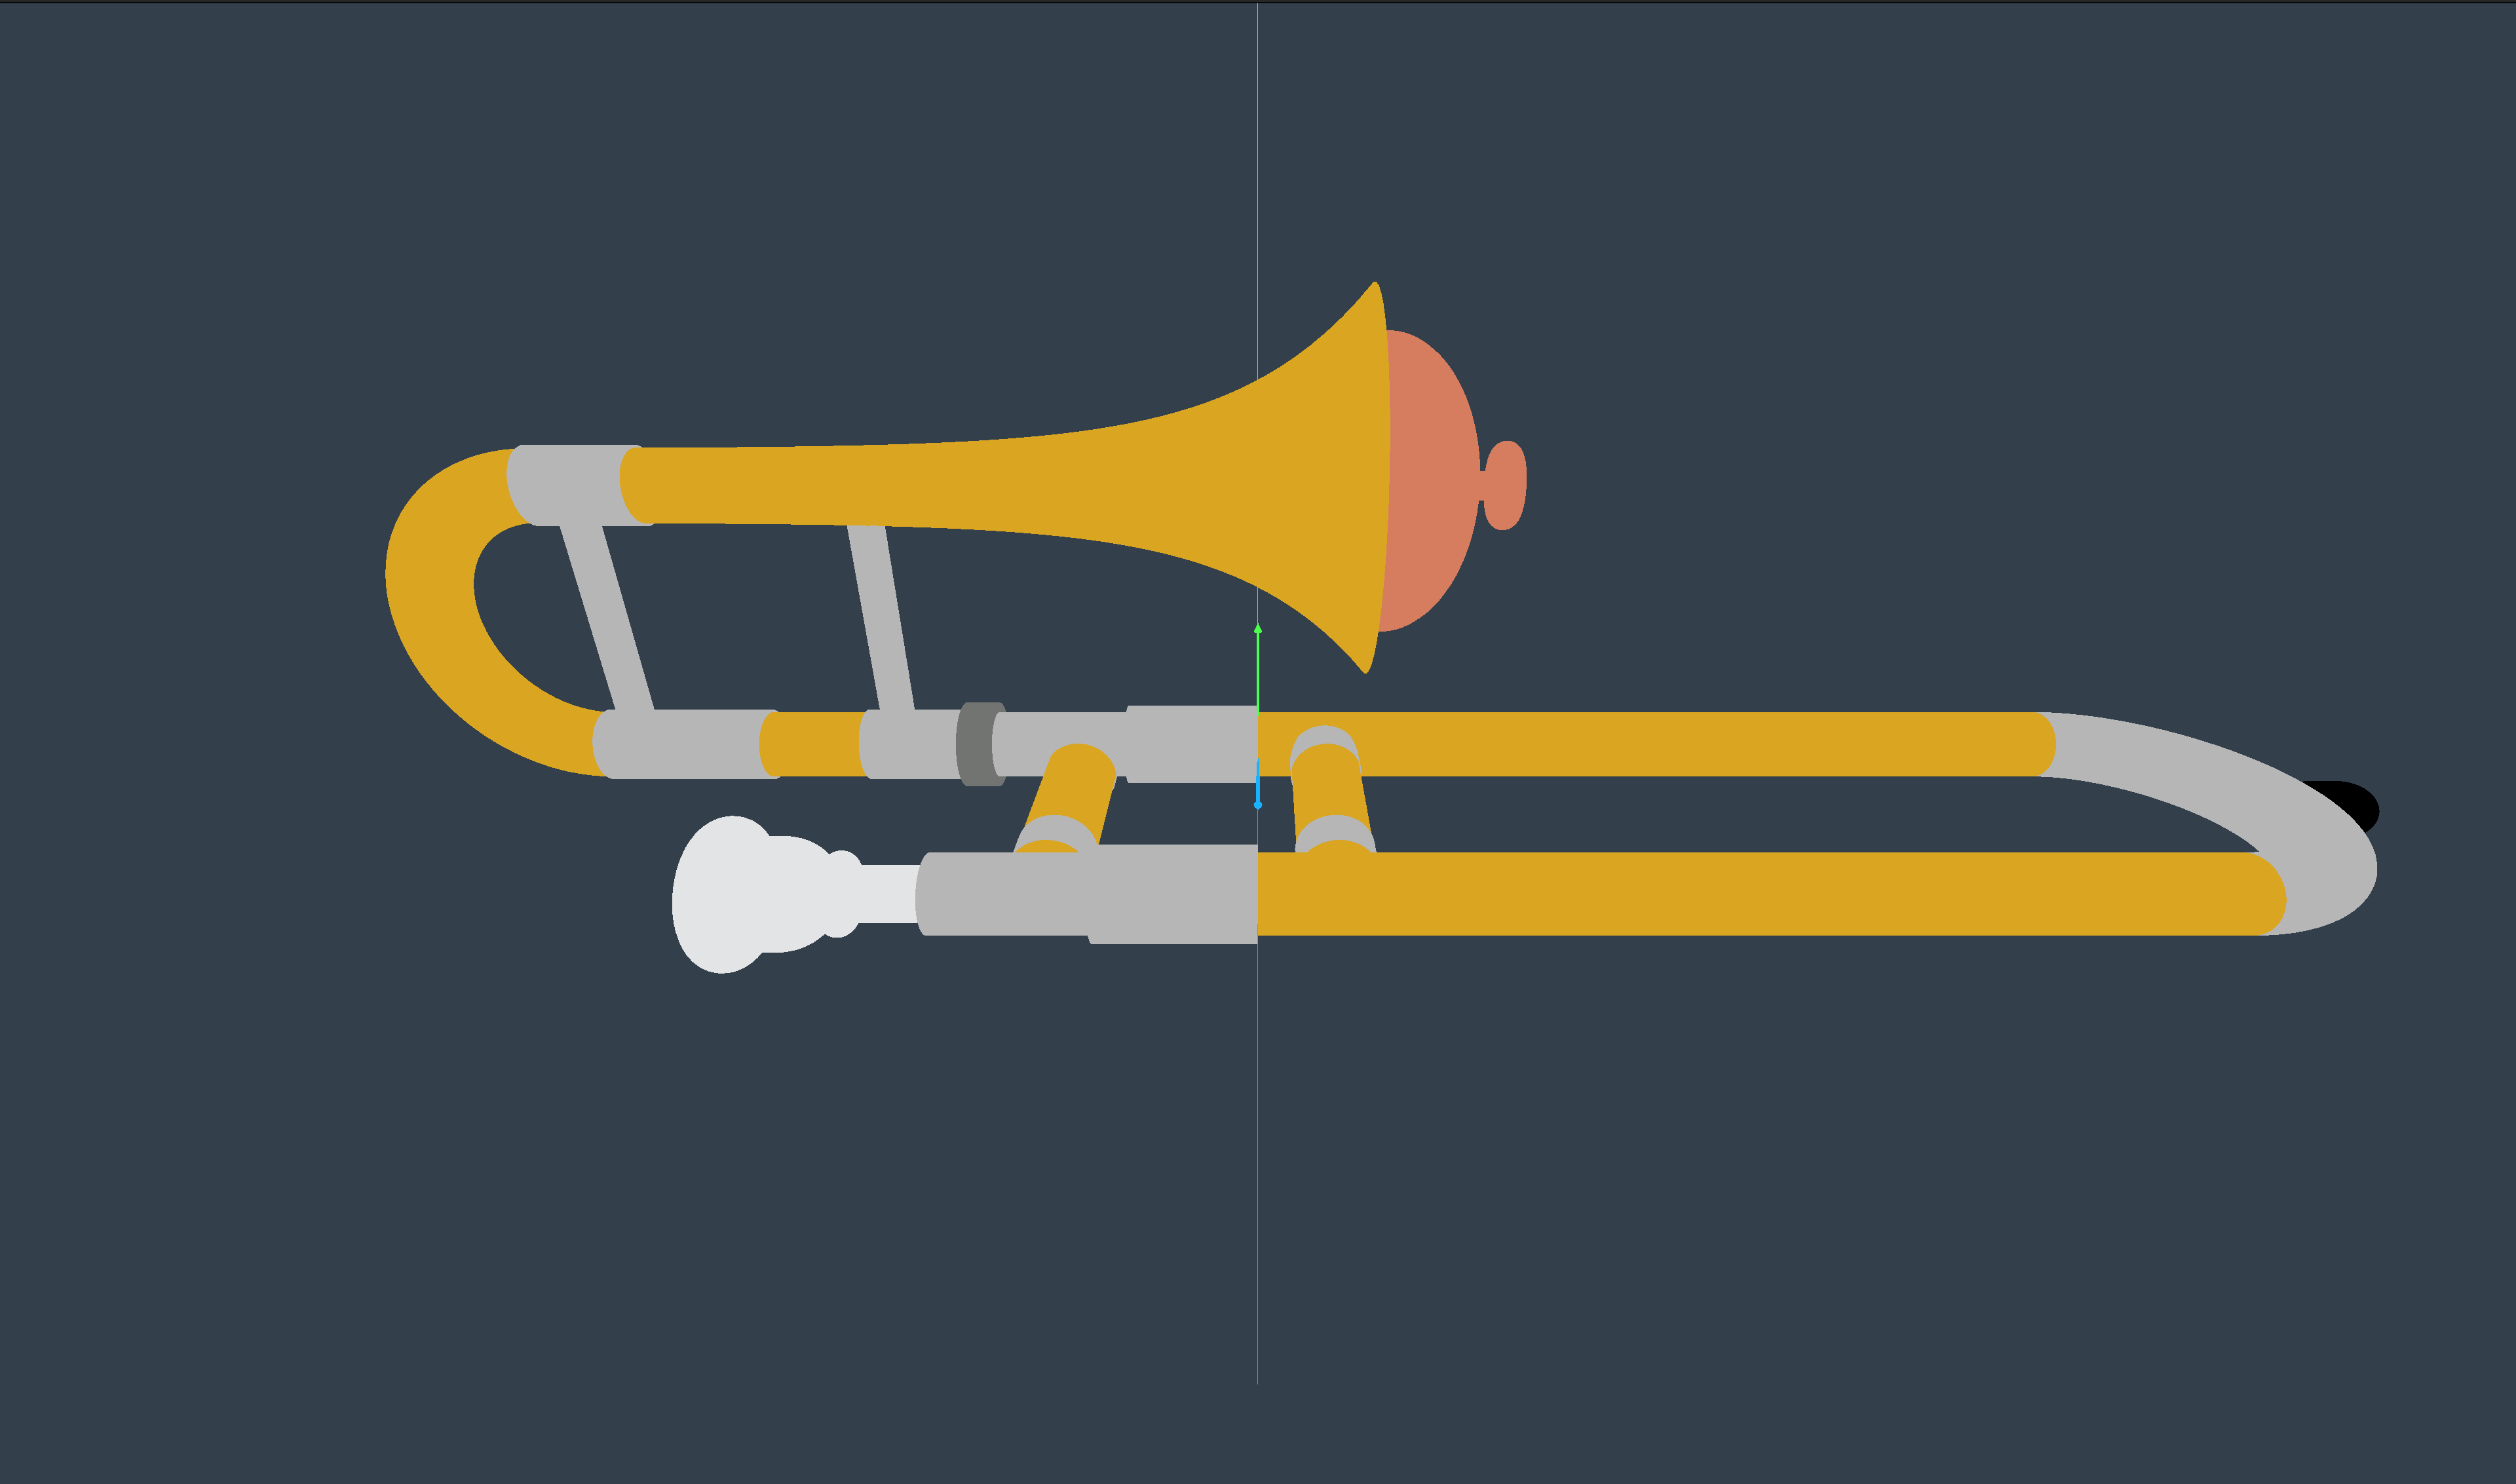
\includegraphics[width=15cm]{resources/img01.png}
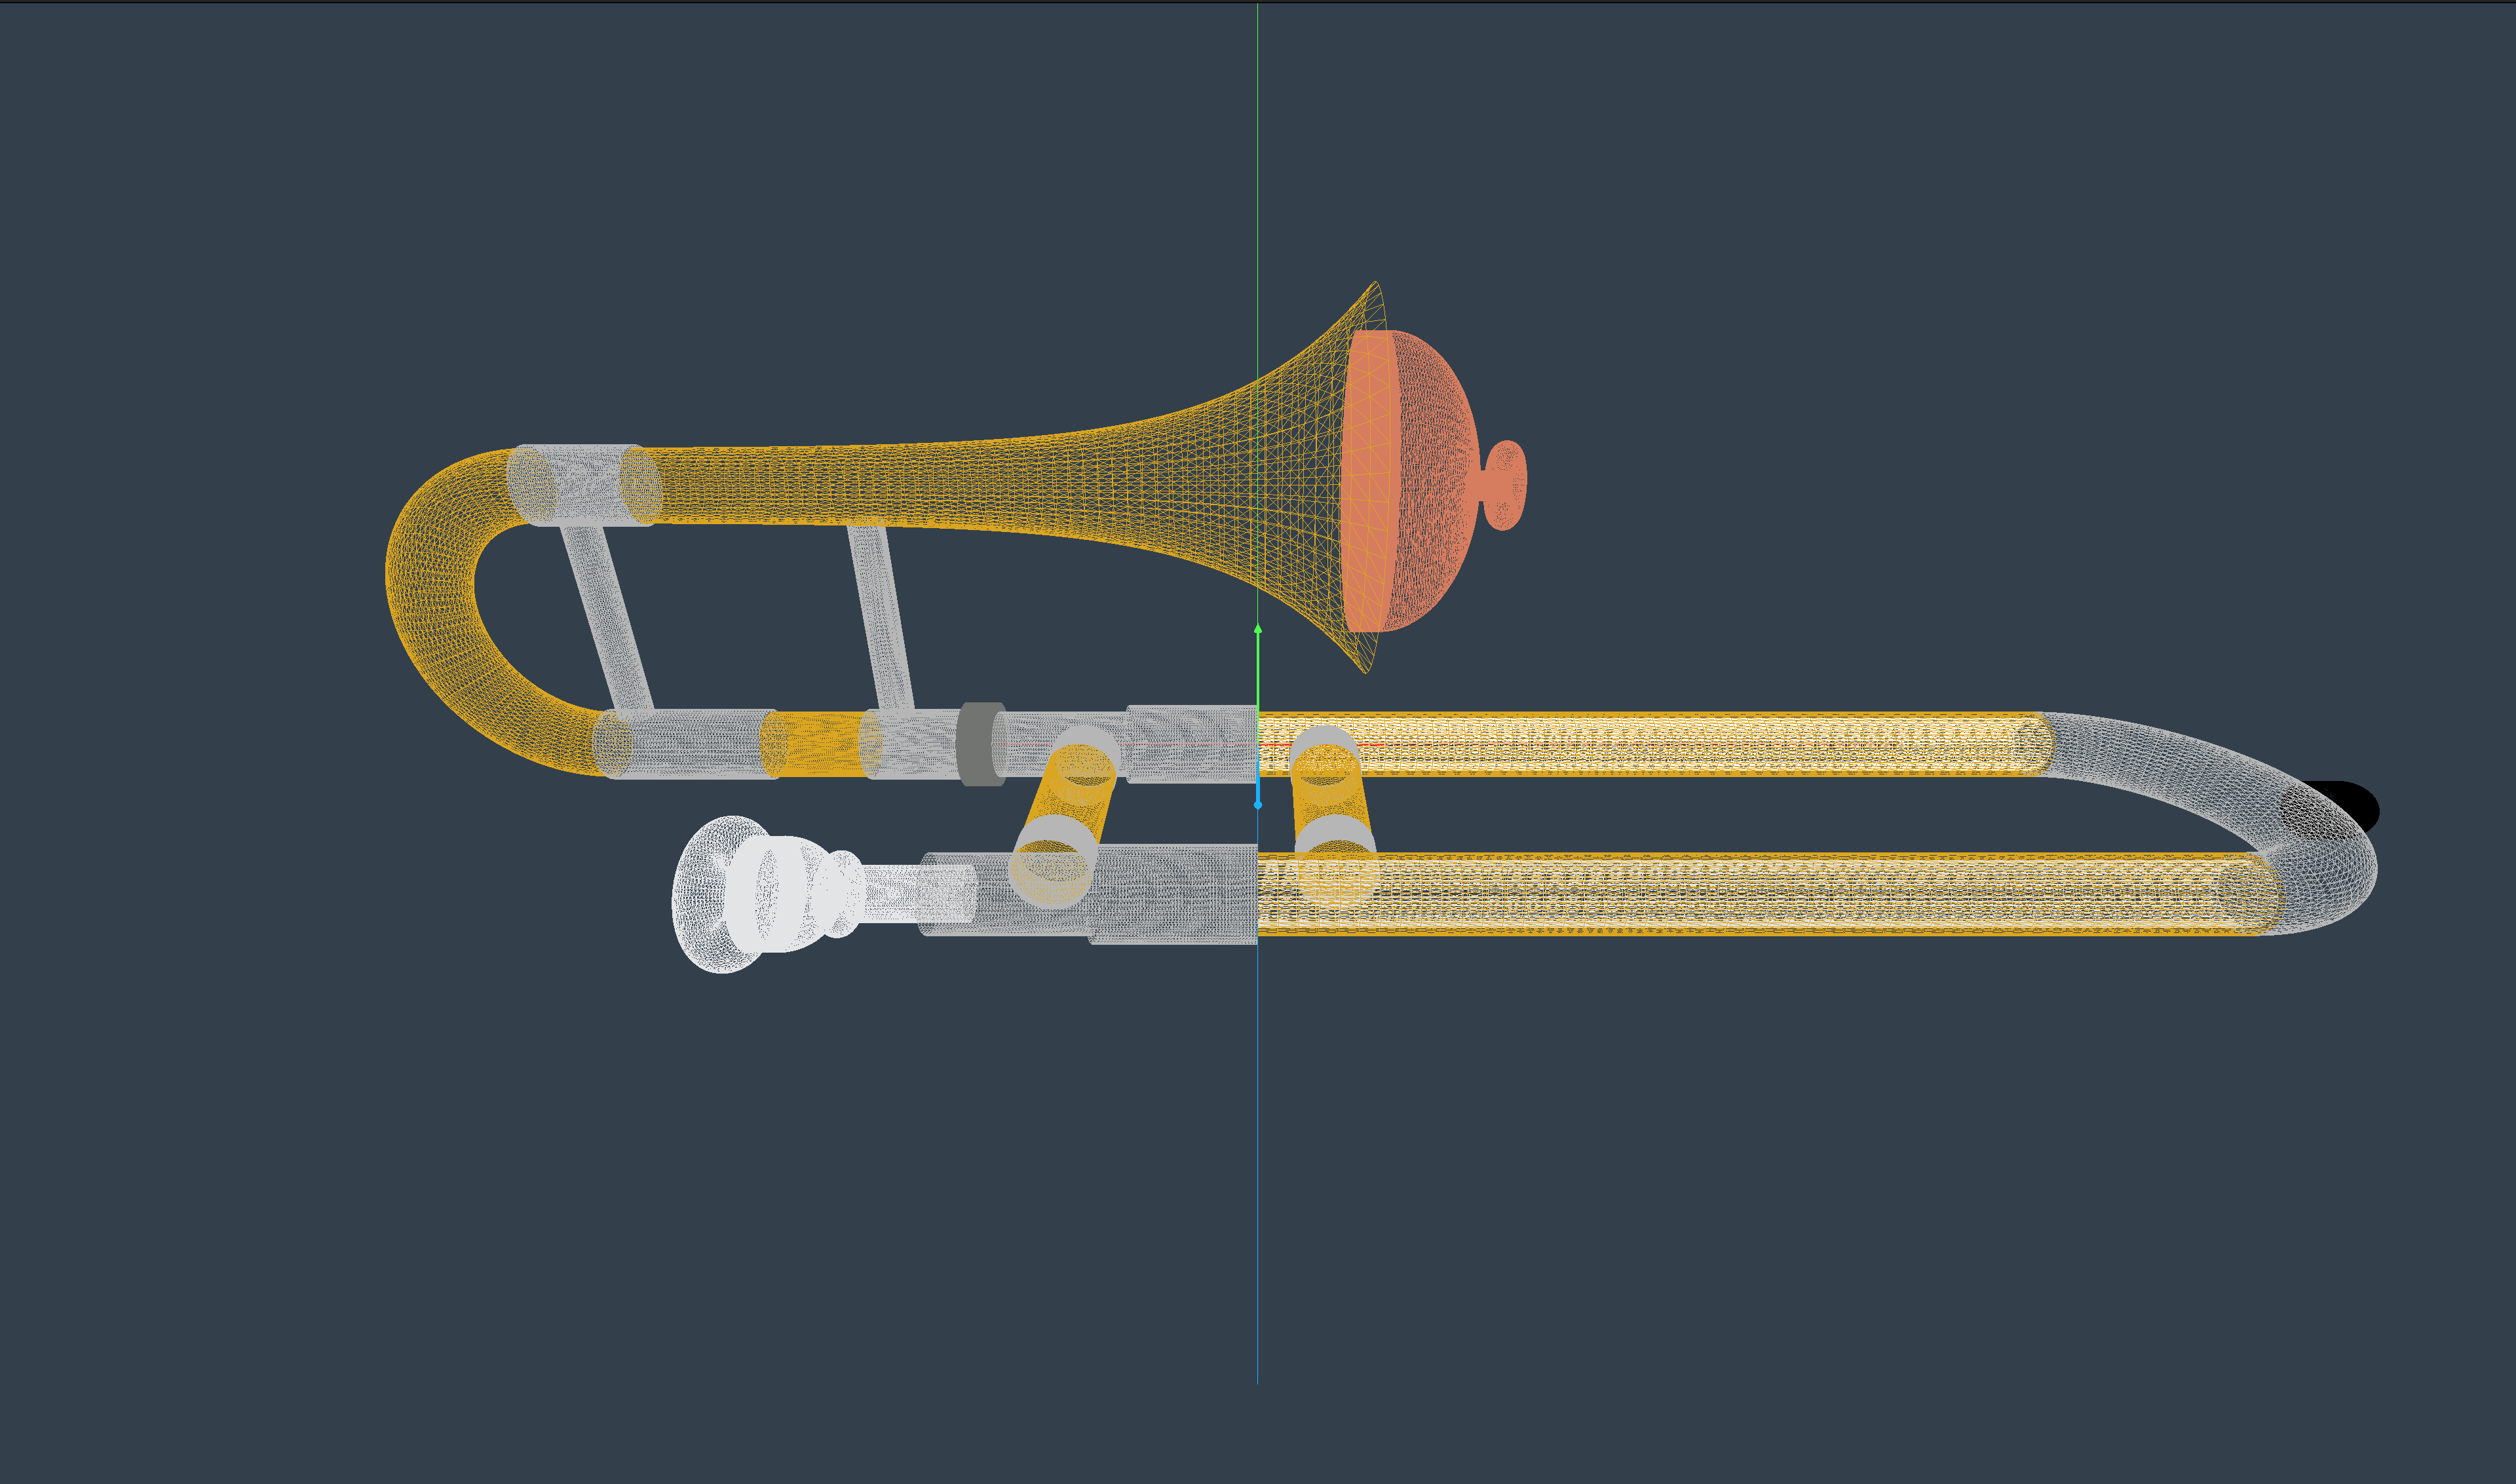
\includegraphics[width=15cm]{resources/img02.png}
\newpage
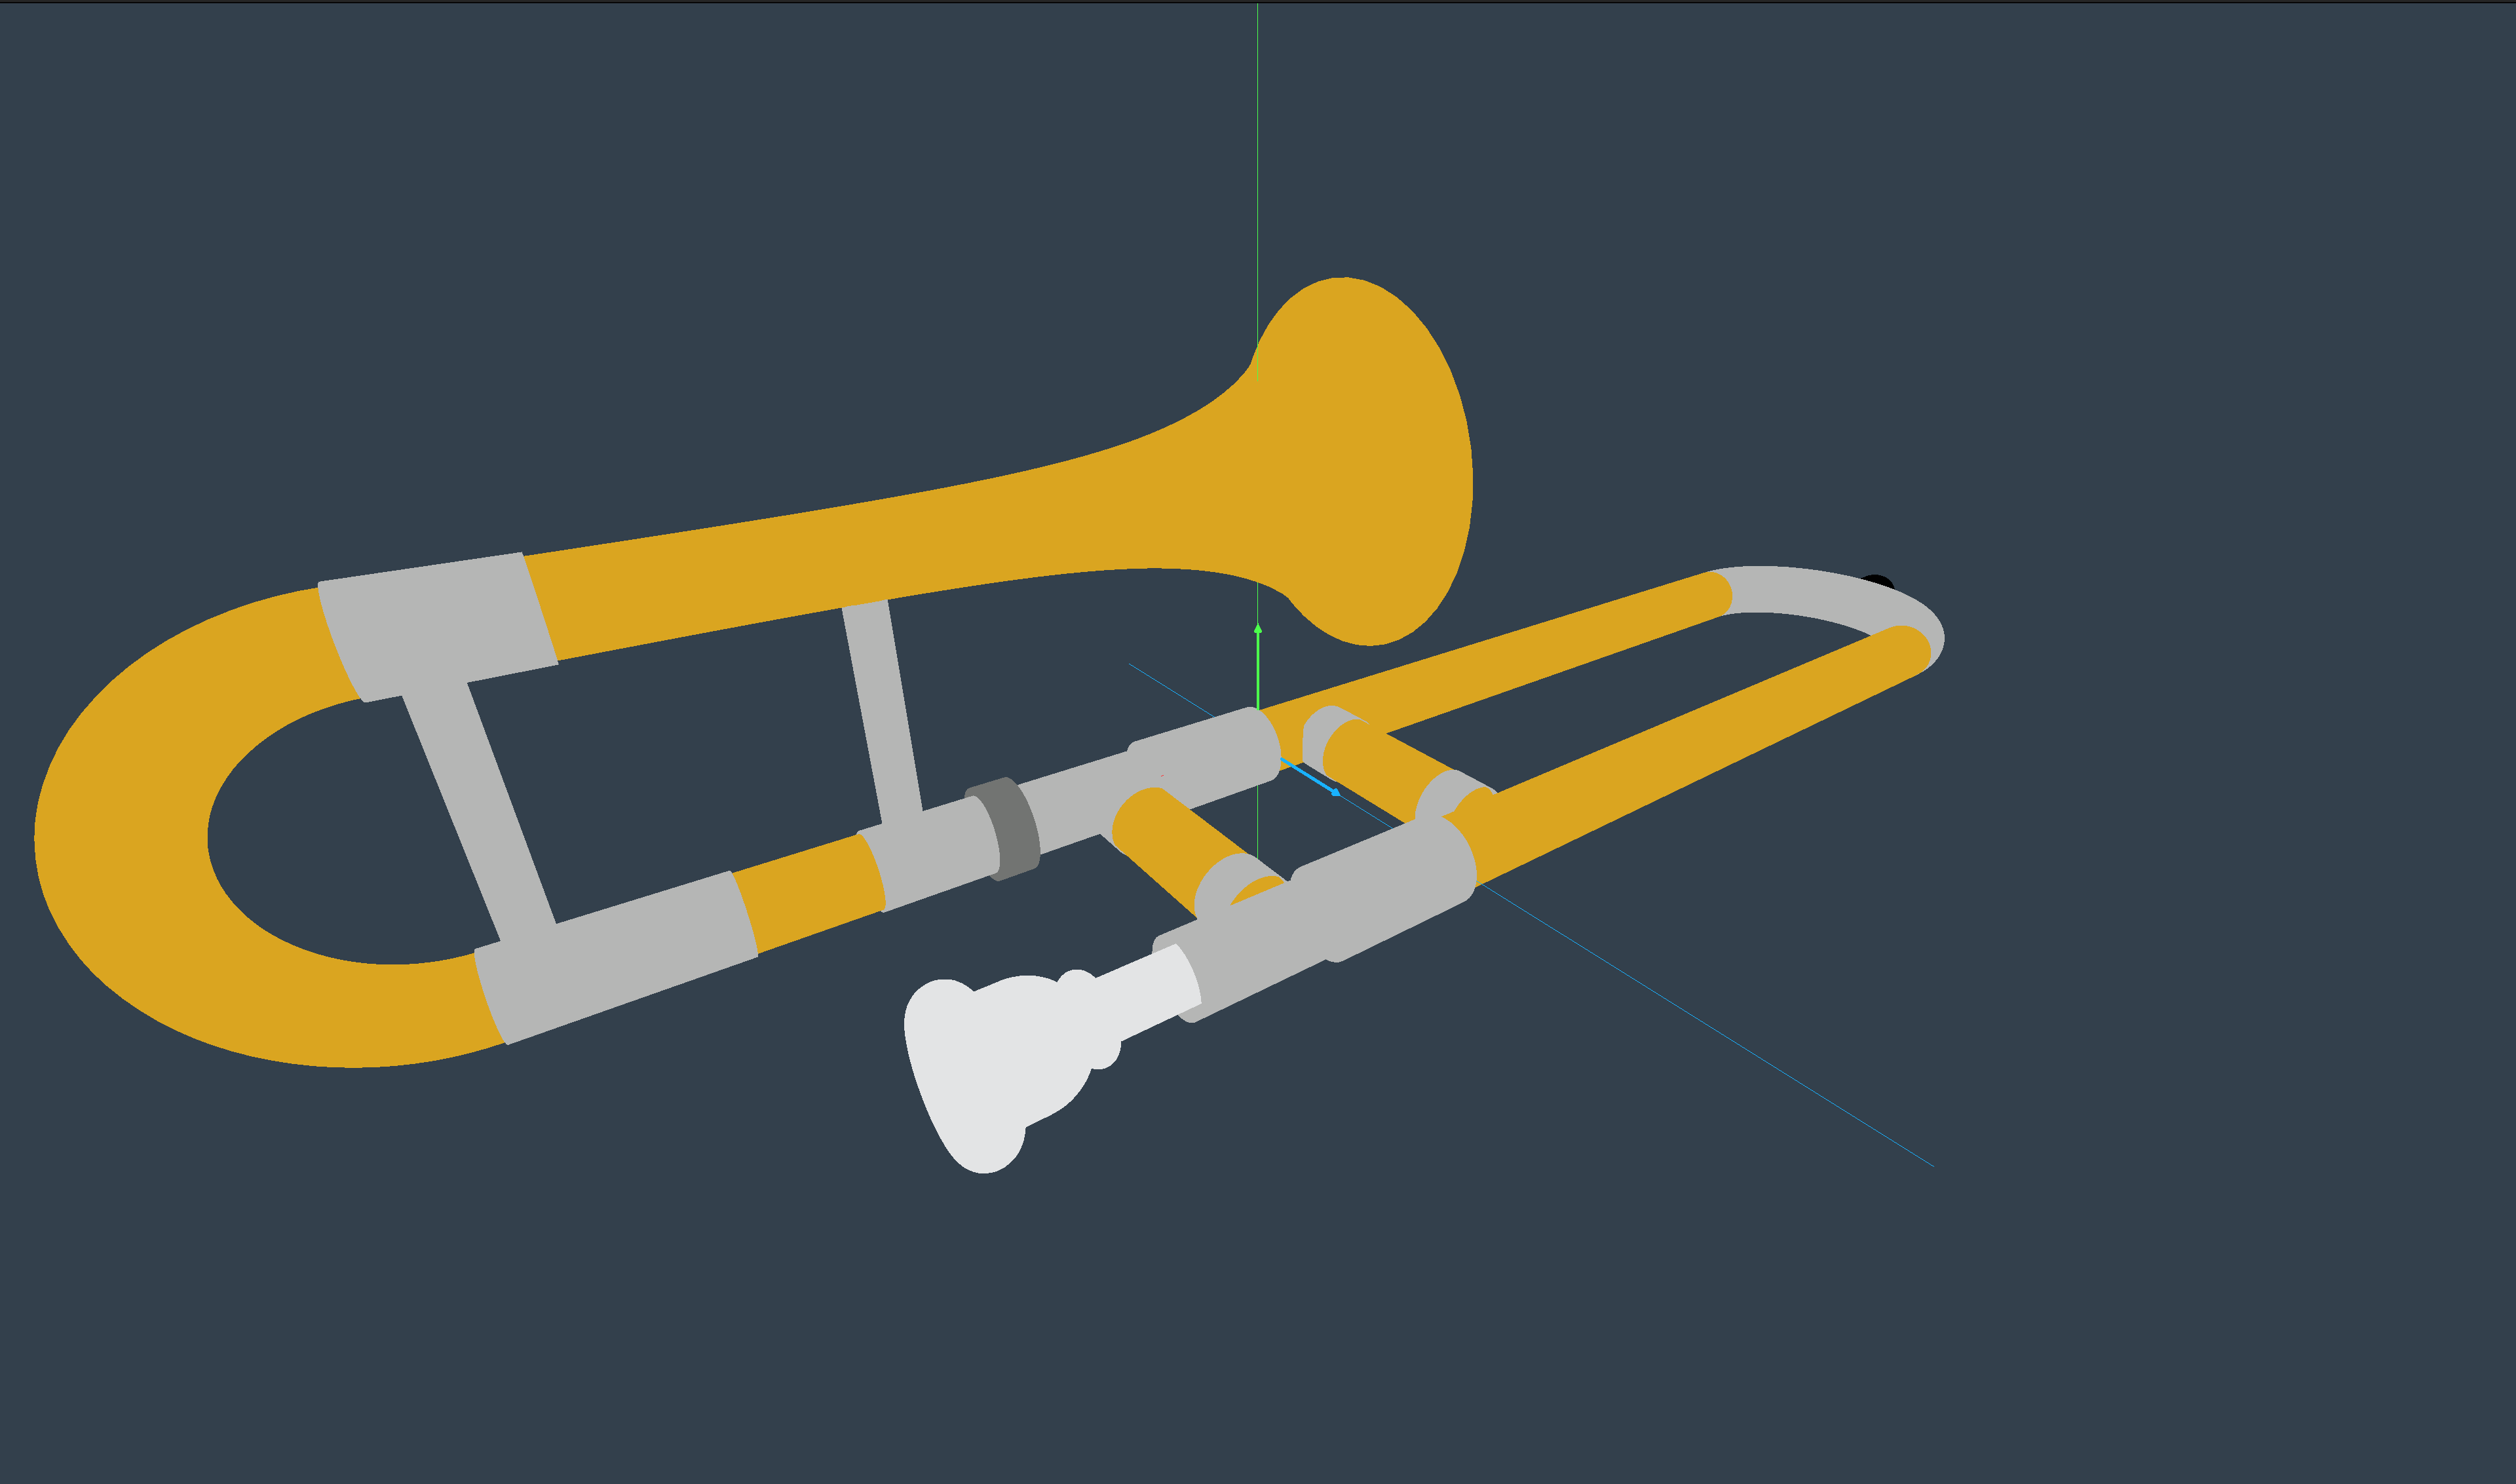
\includegraphics[width=15cm]{resources/img03.png}
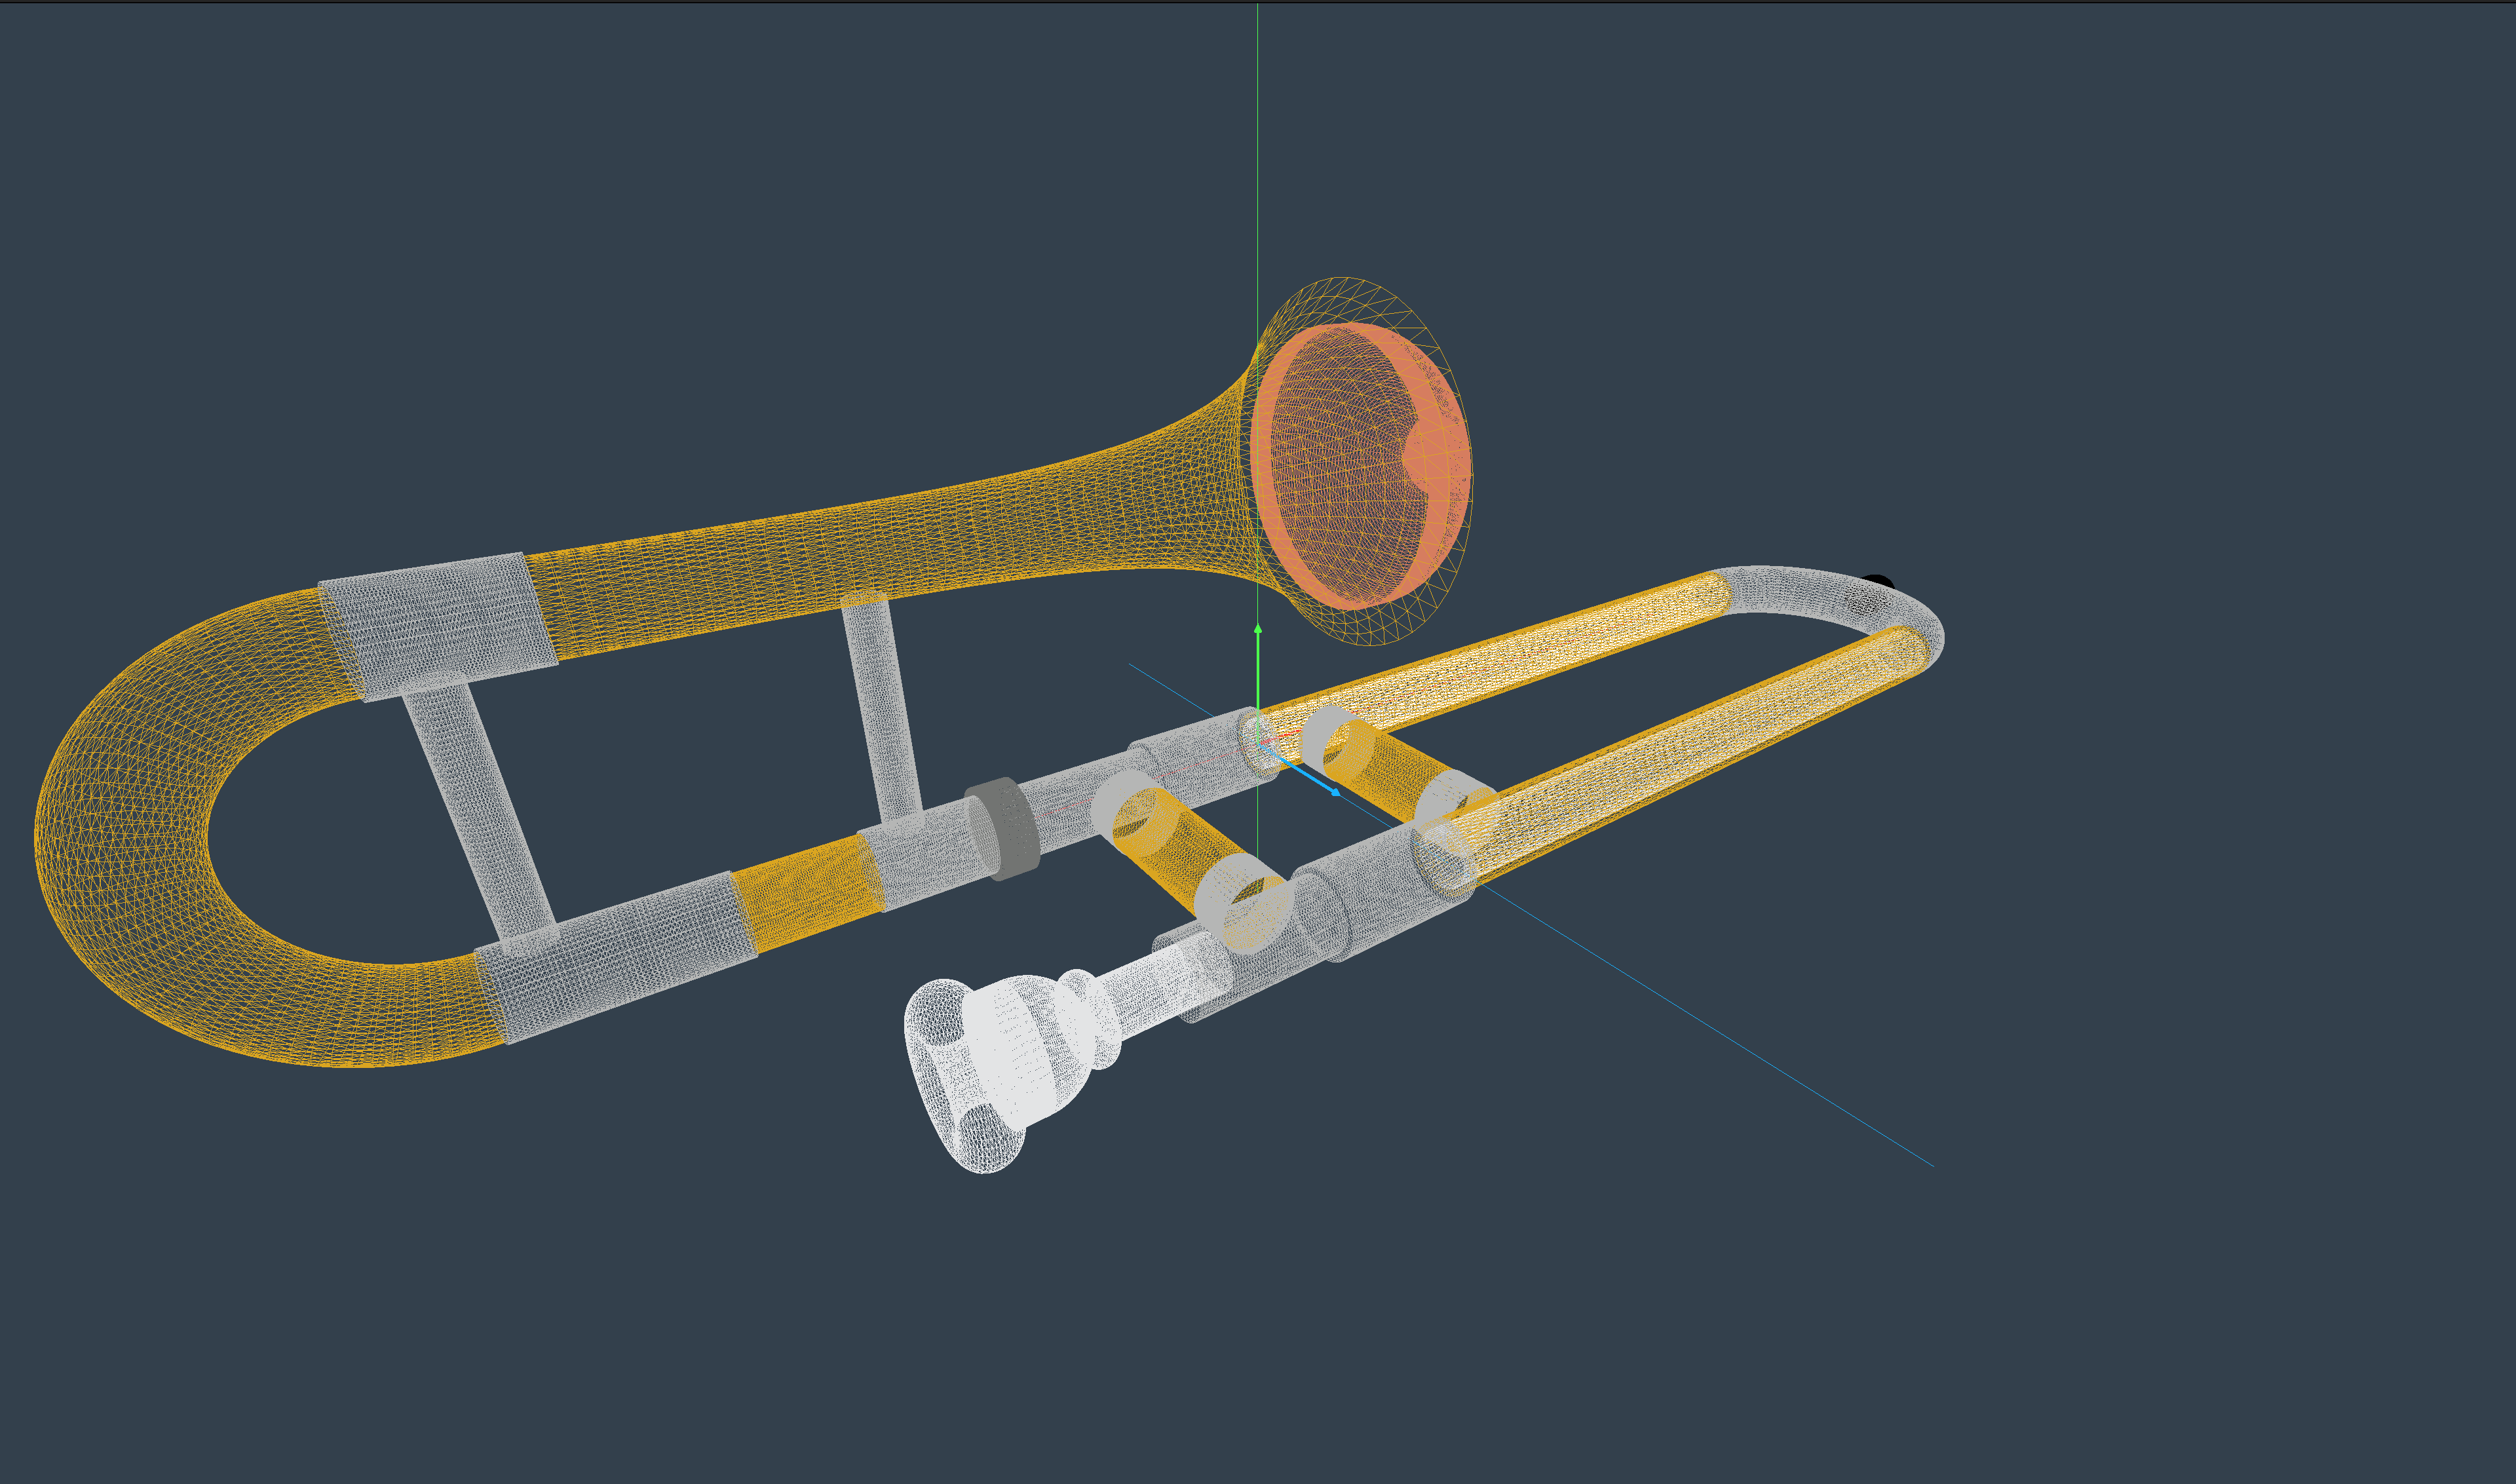
\includegraphics[width=15cm]{resources/img04.png}
\newpage
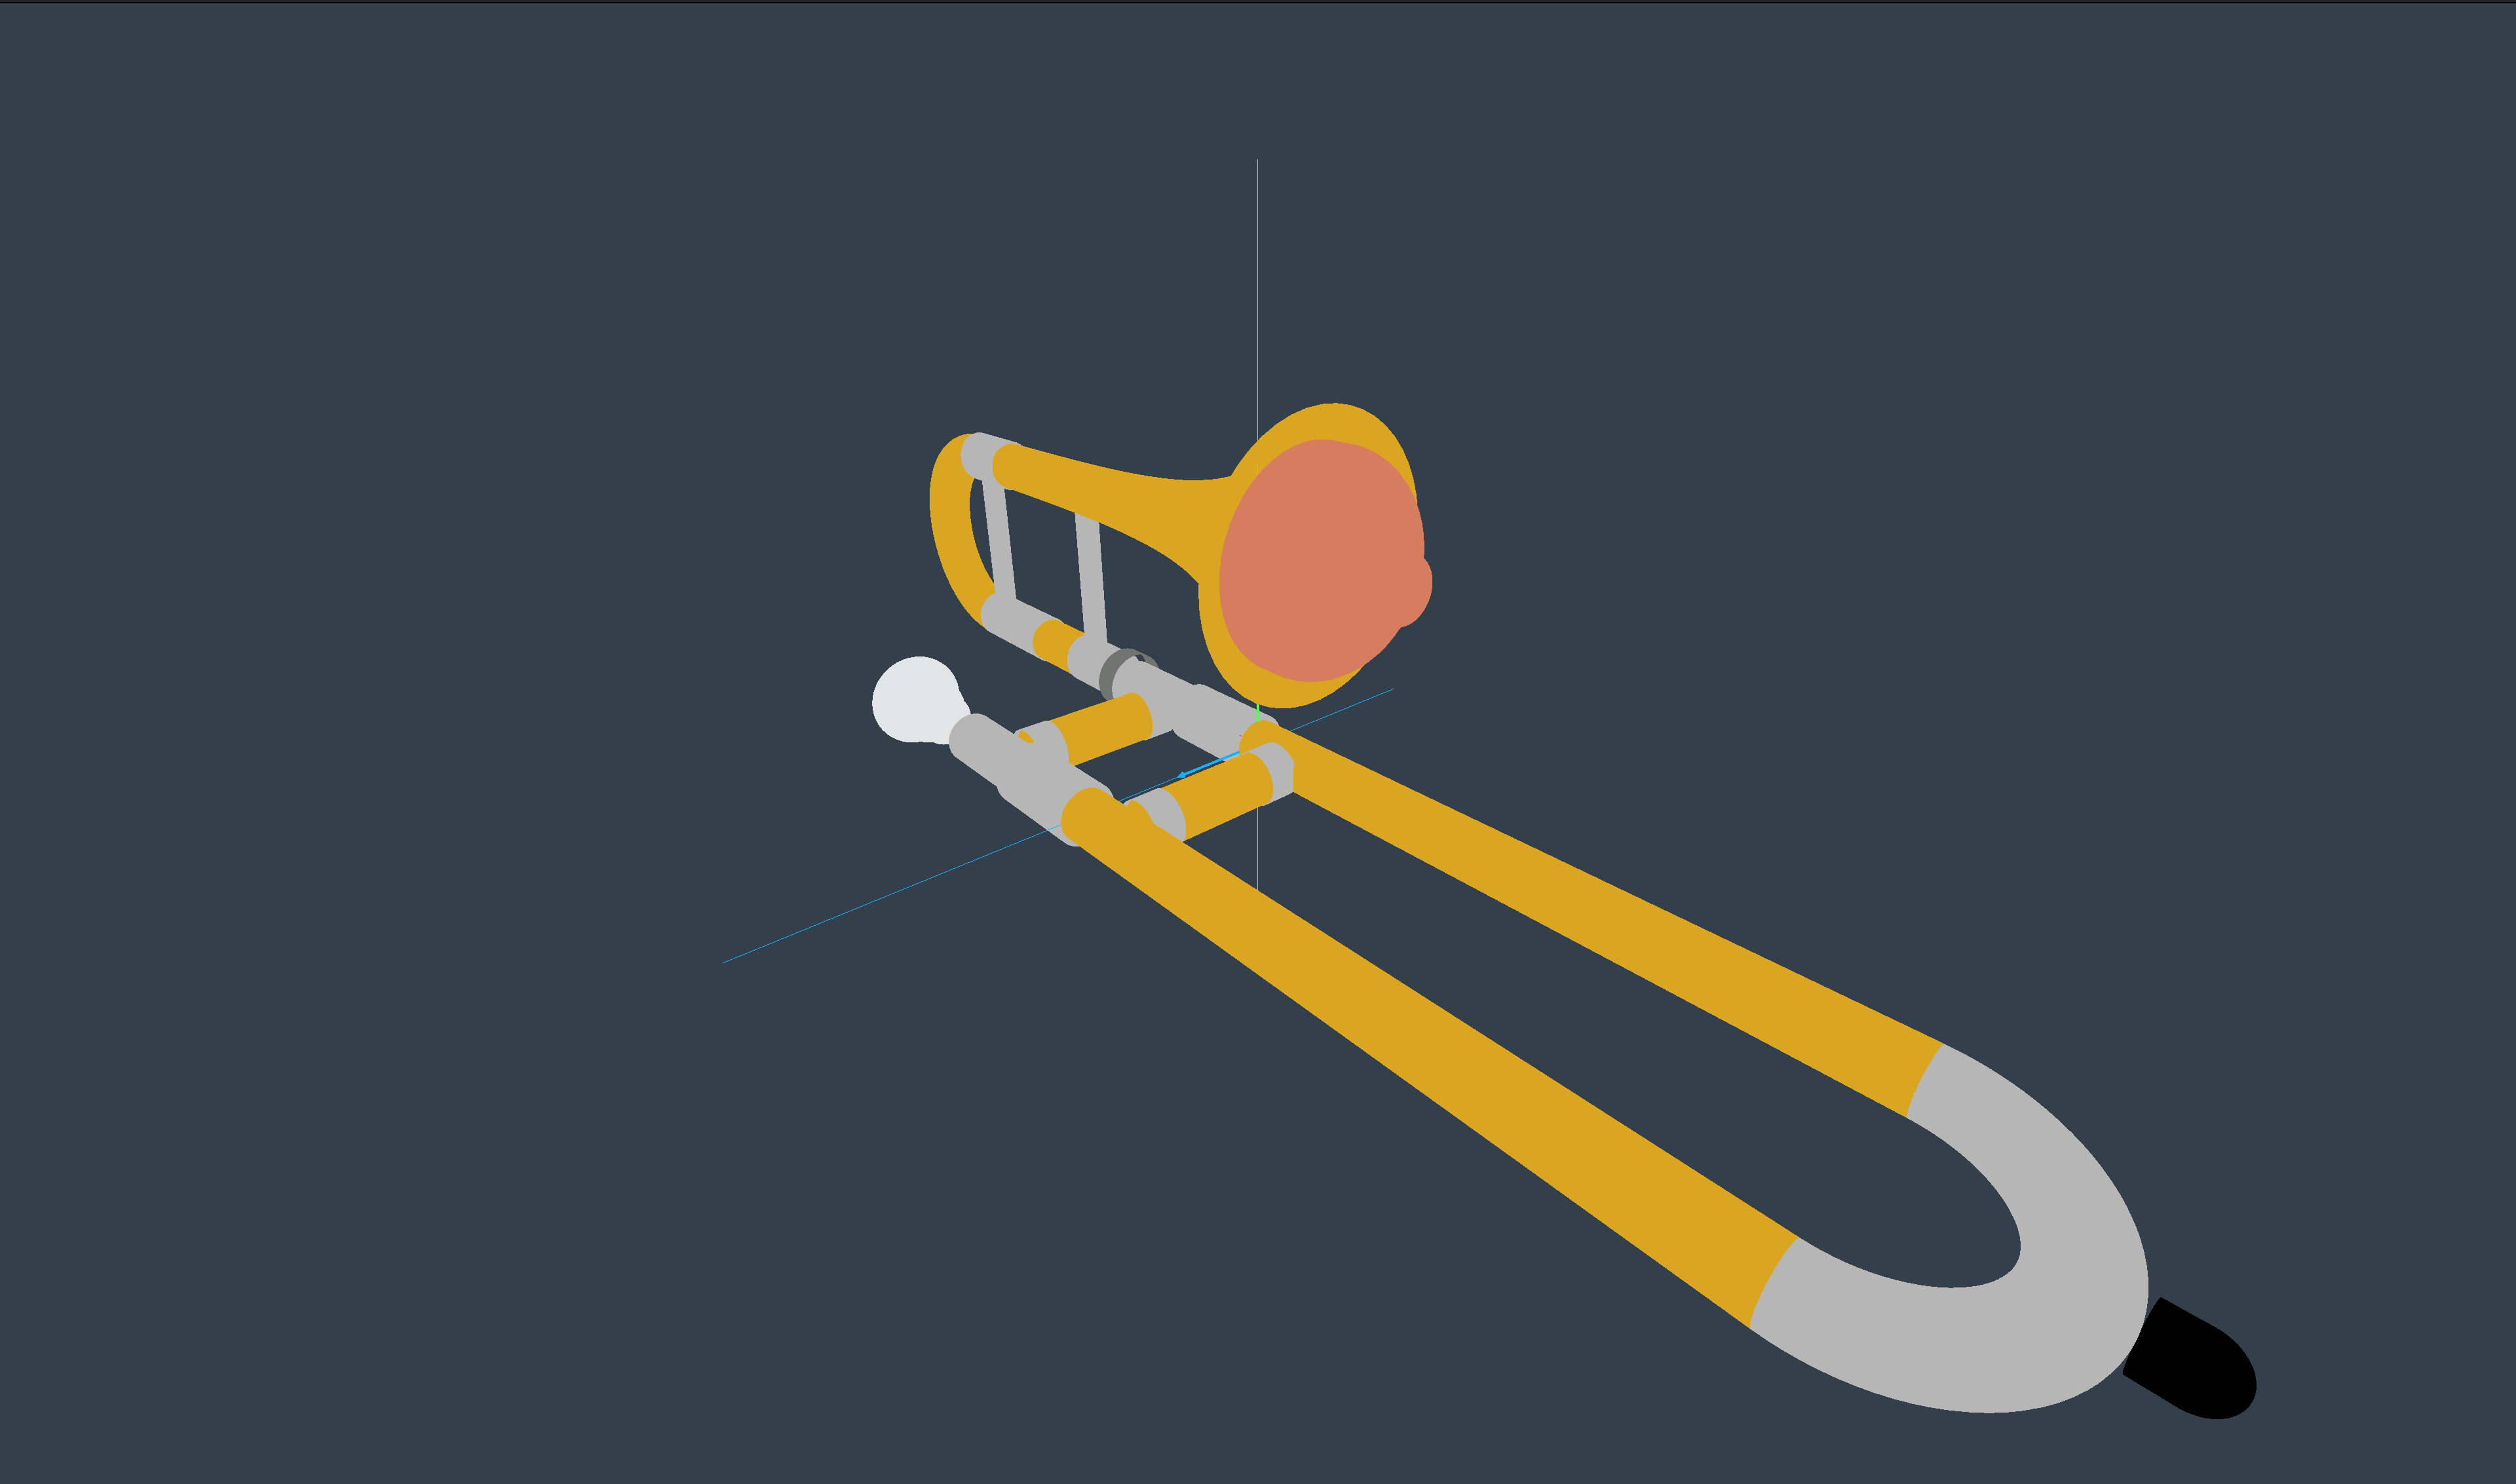
\includegraphics[width=15cm]{resources/img05.png}
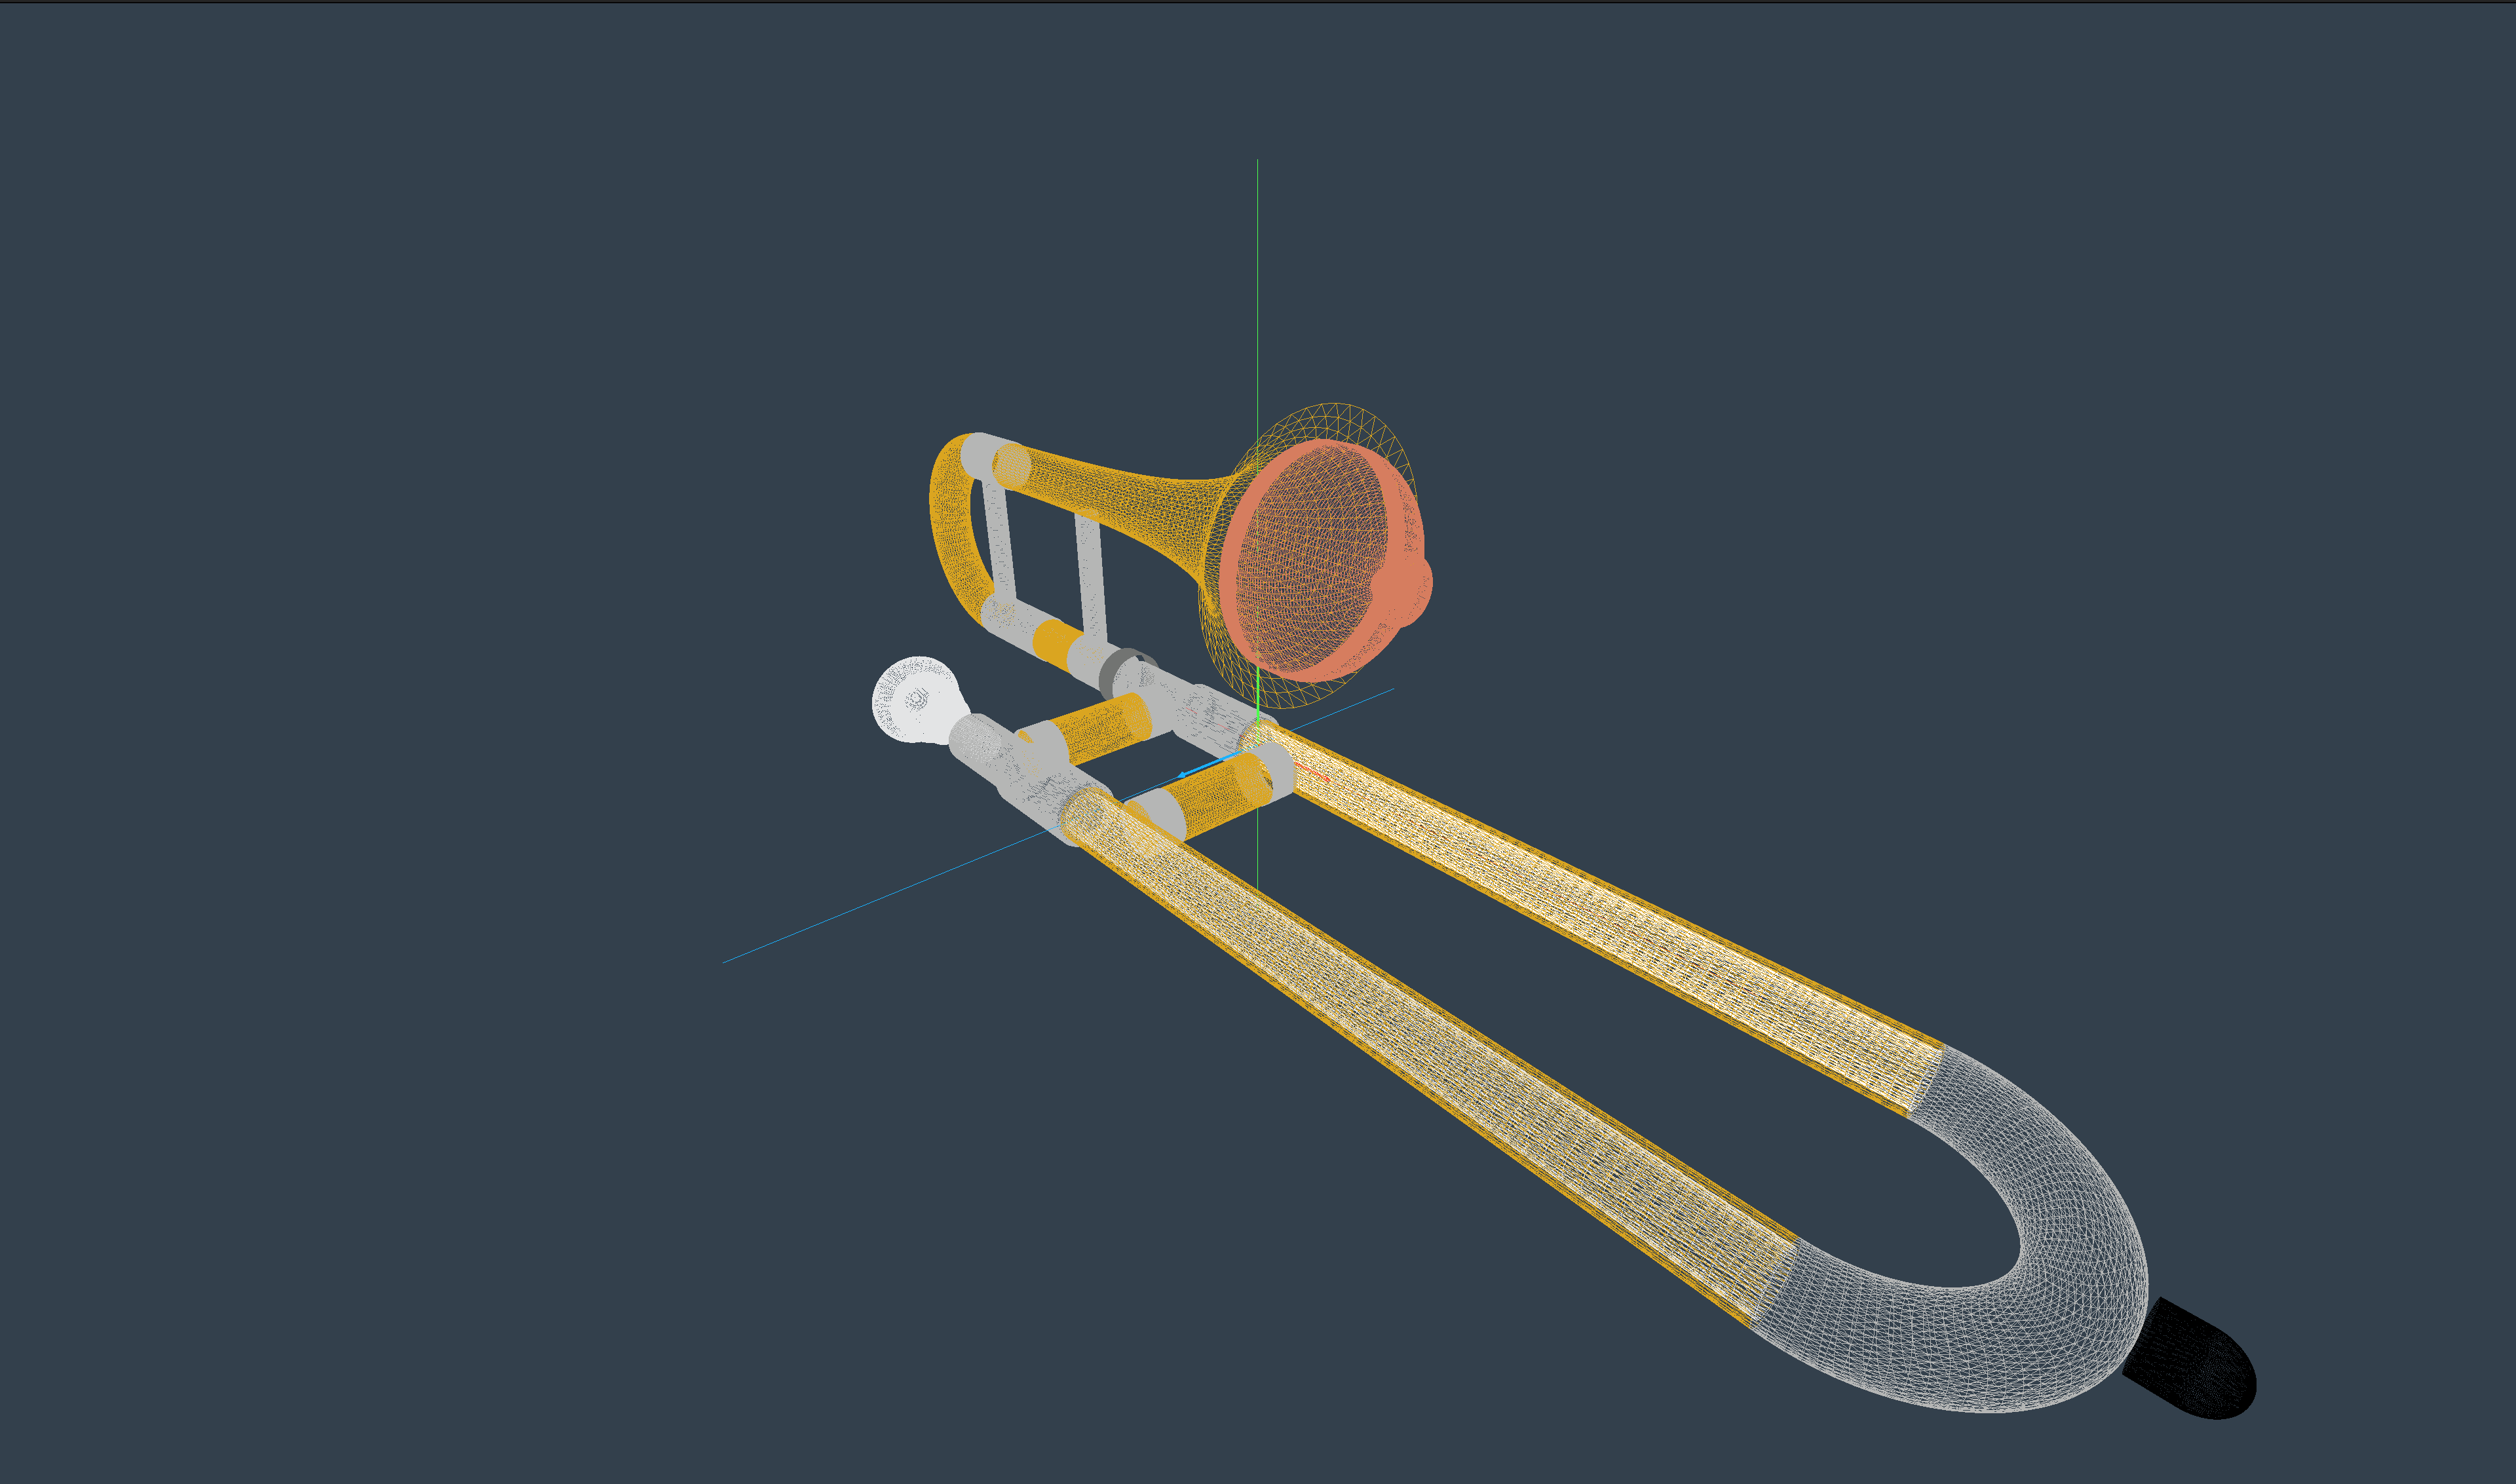
\includegraphics[width=15cm]{resources/img06.png}
\newpage
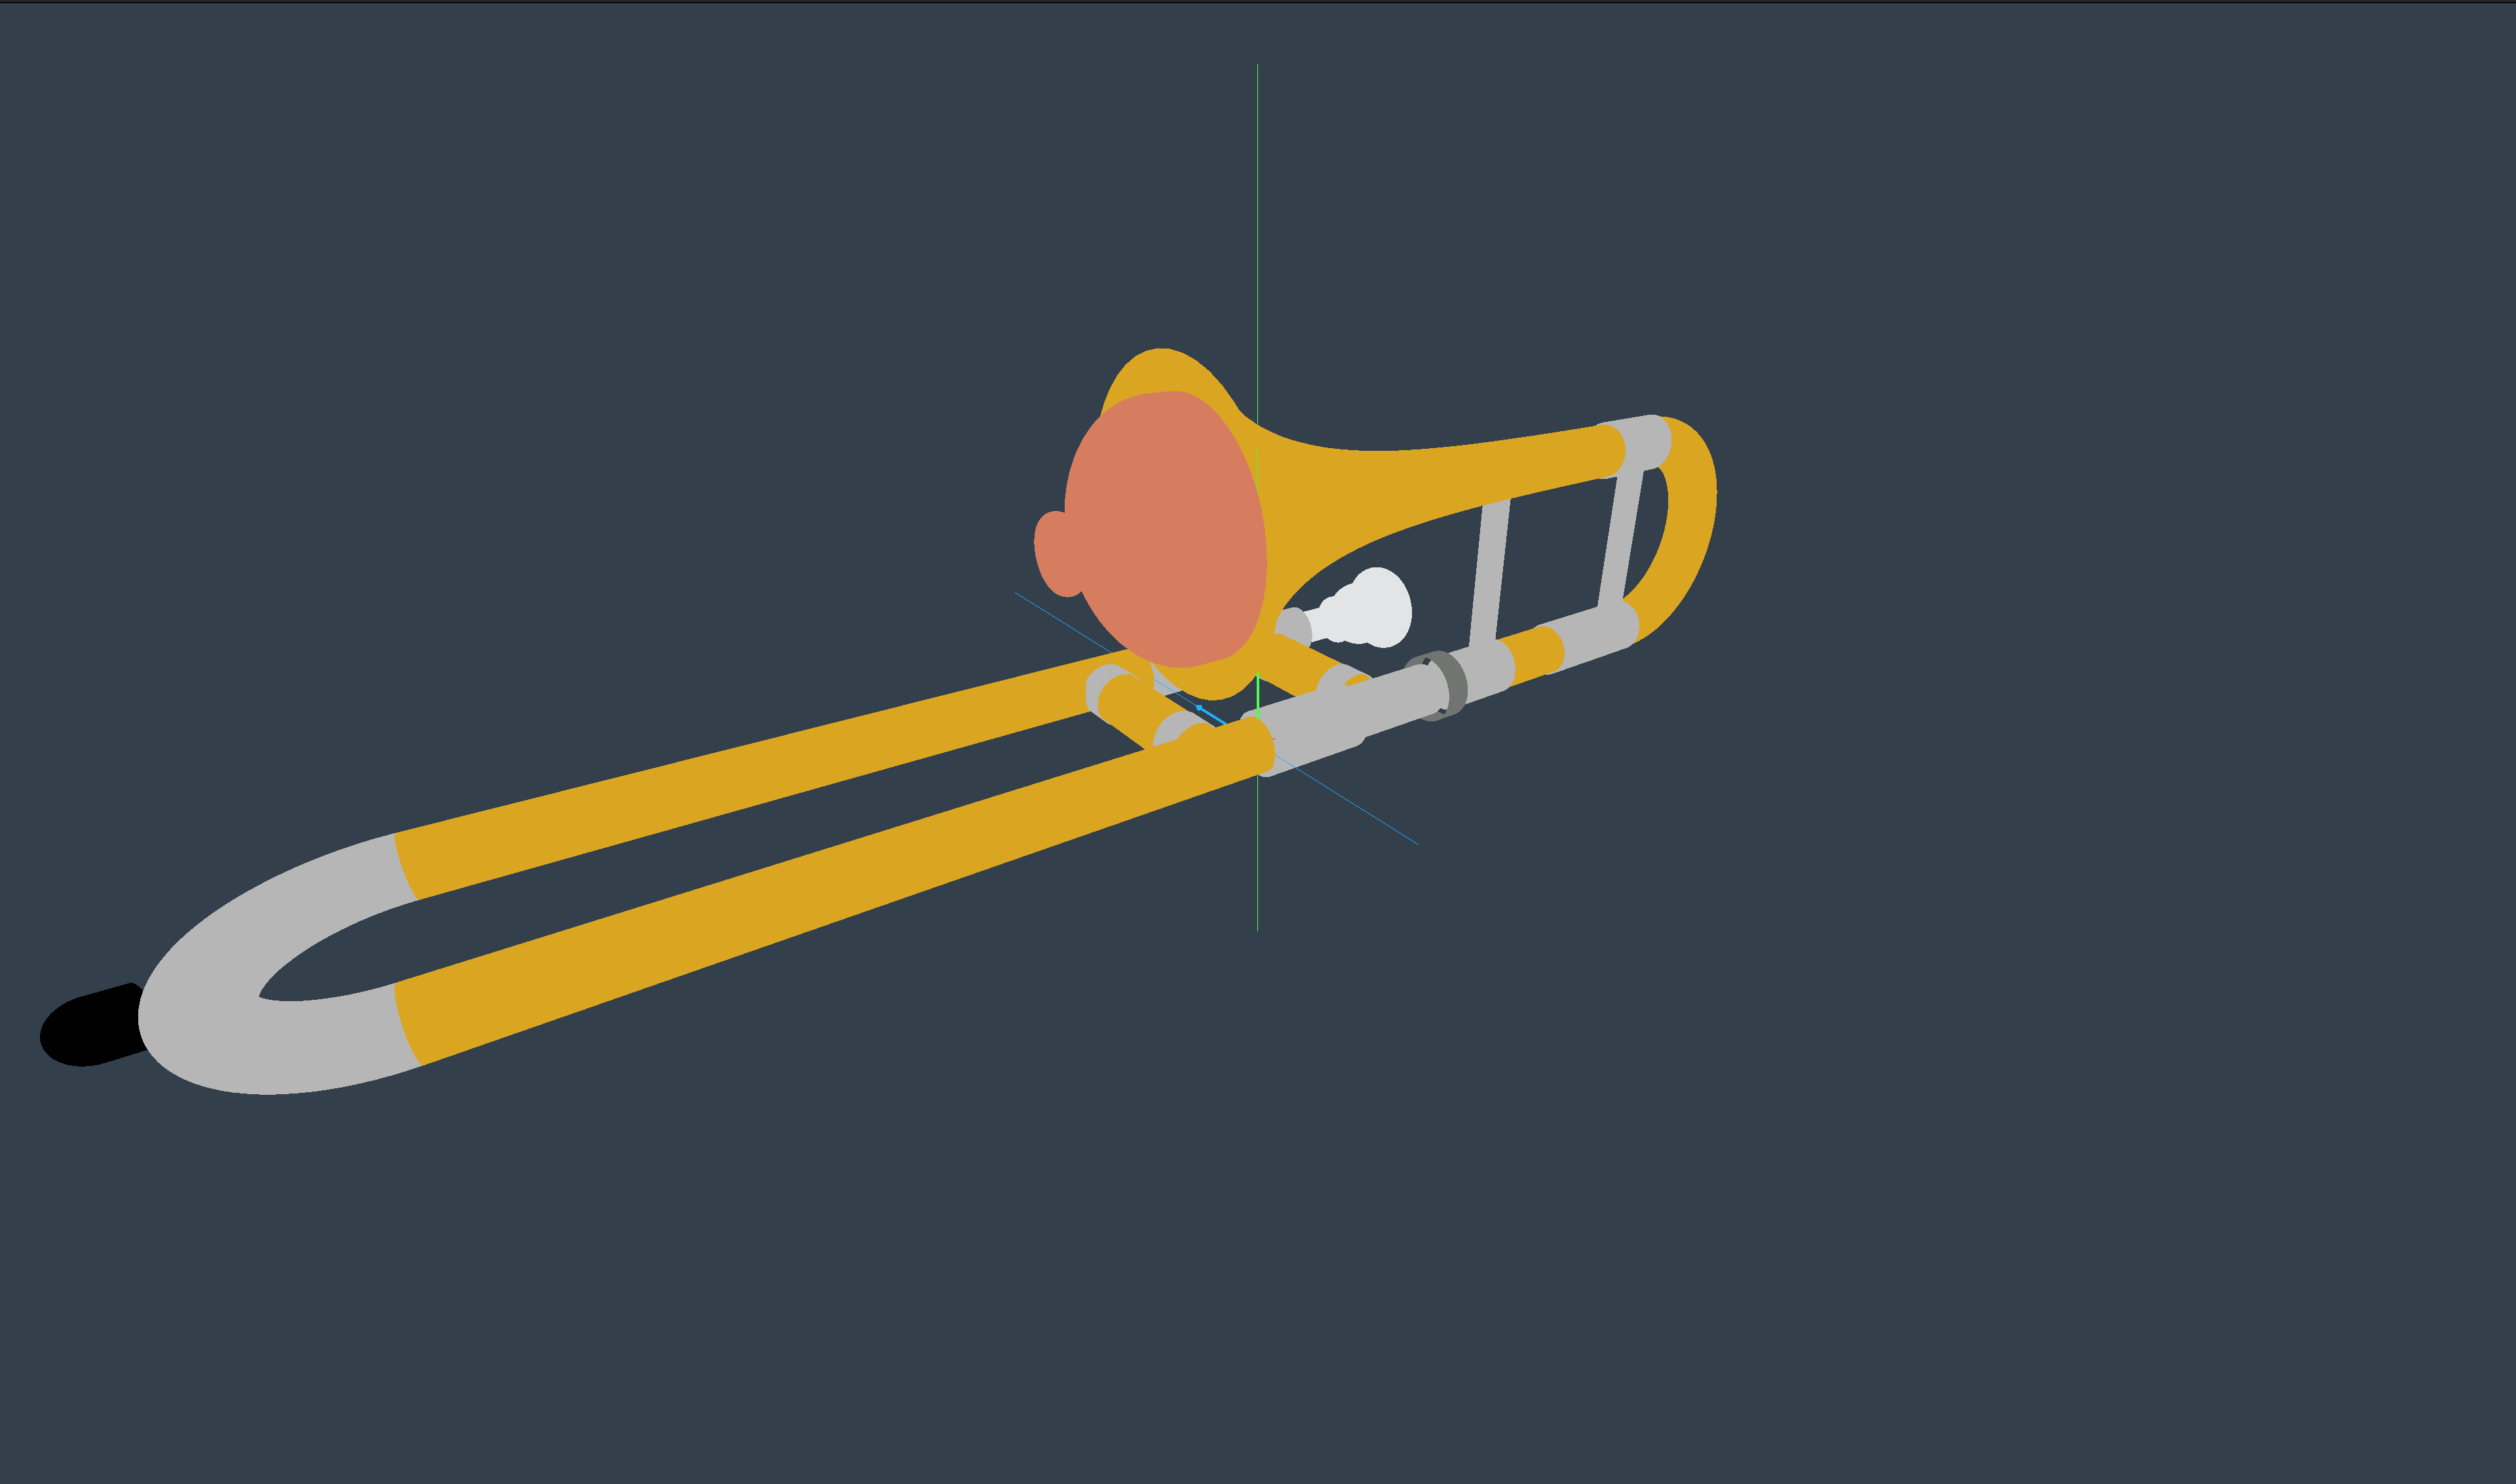
\includegraphics[width=15cm]{resources/img07.png}
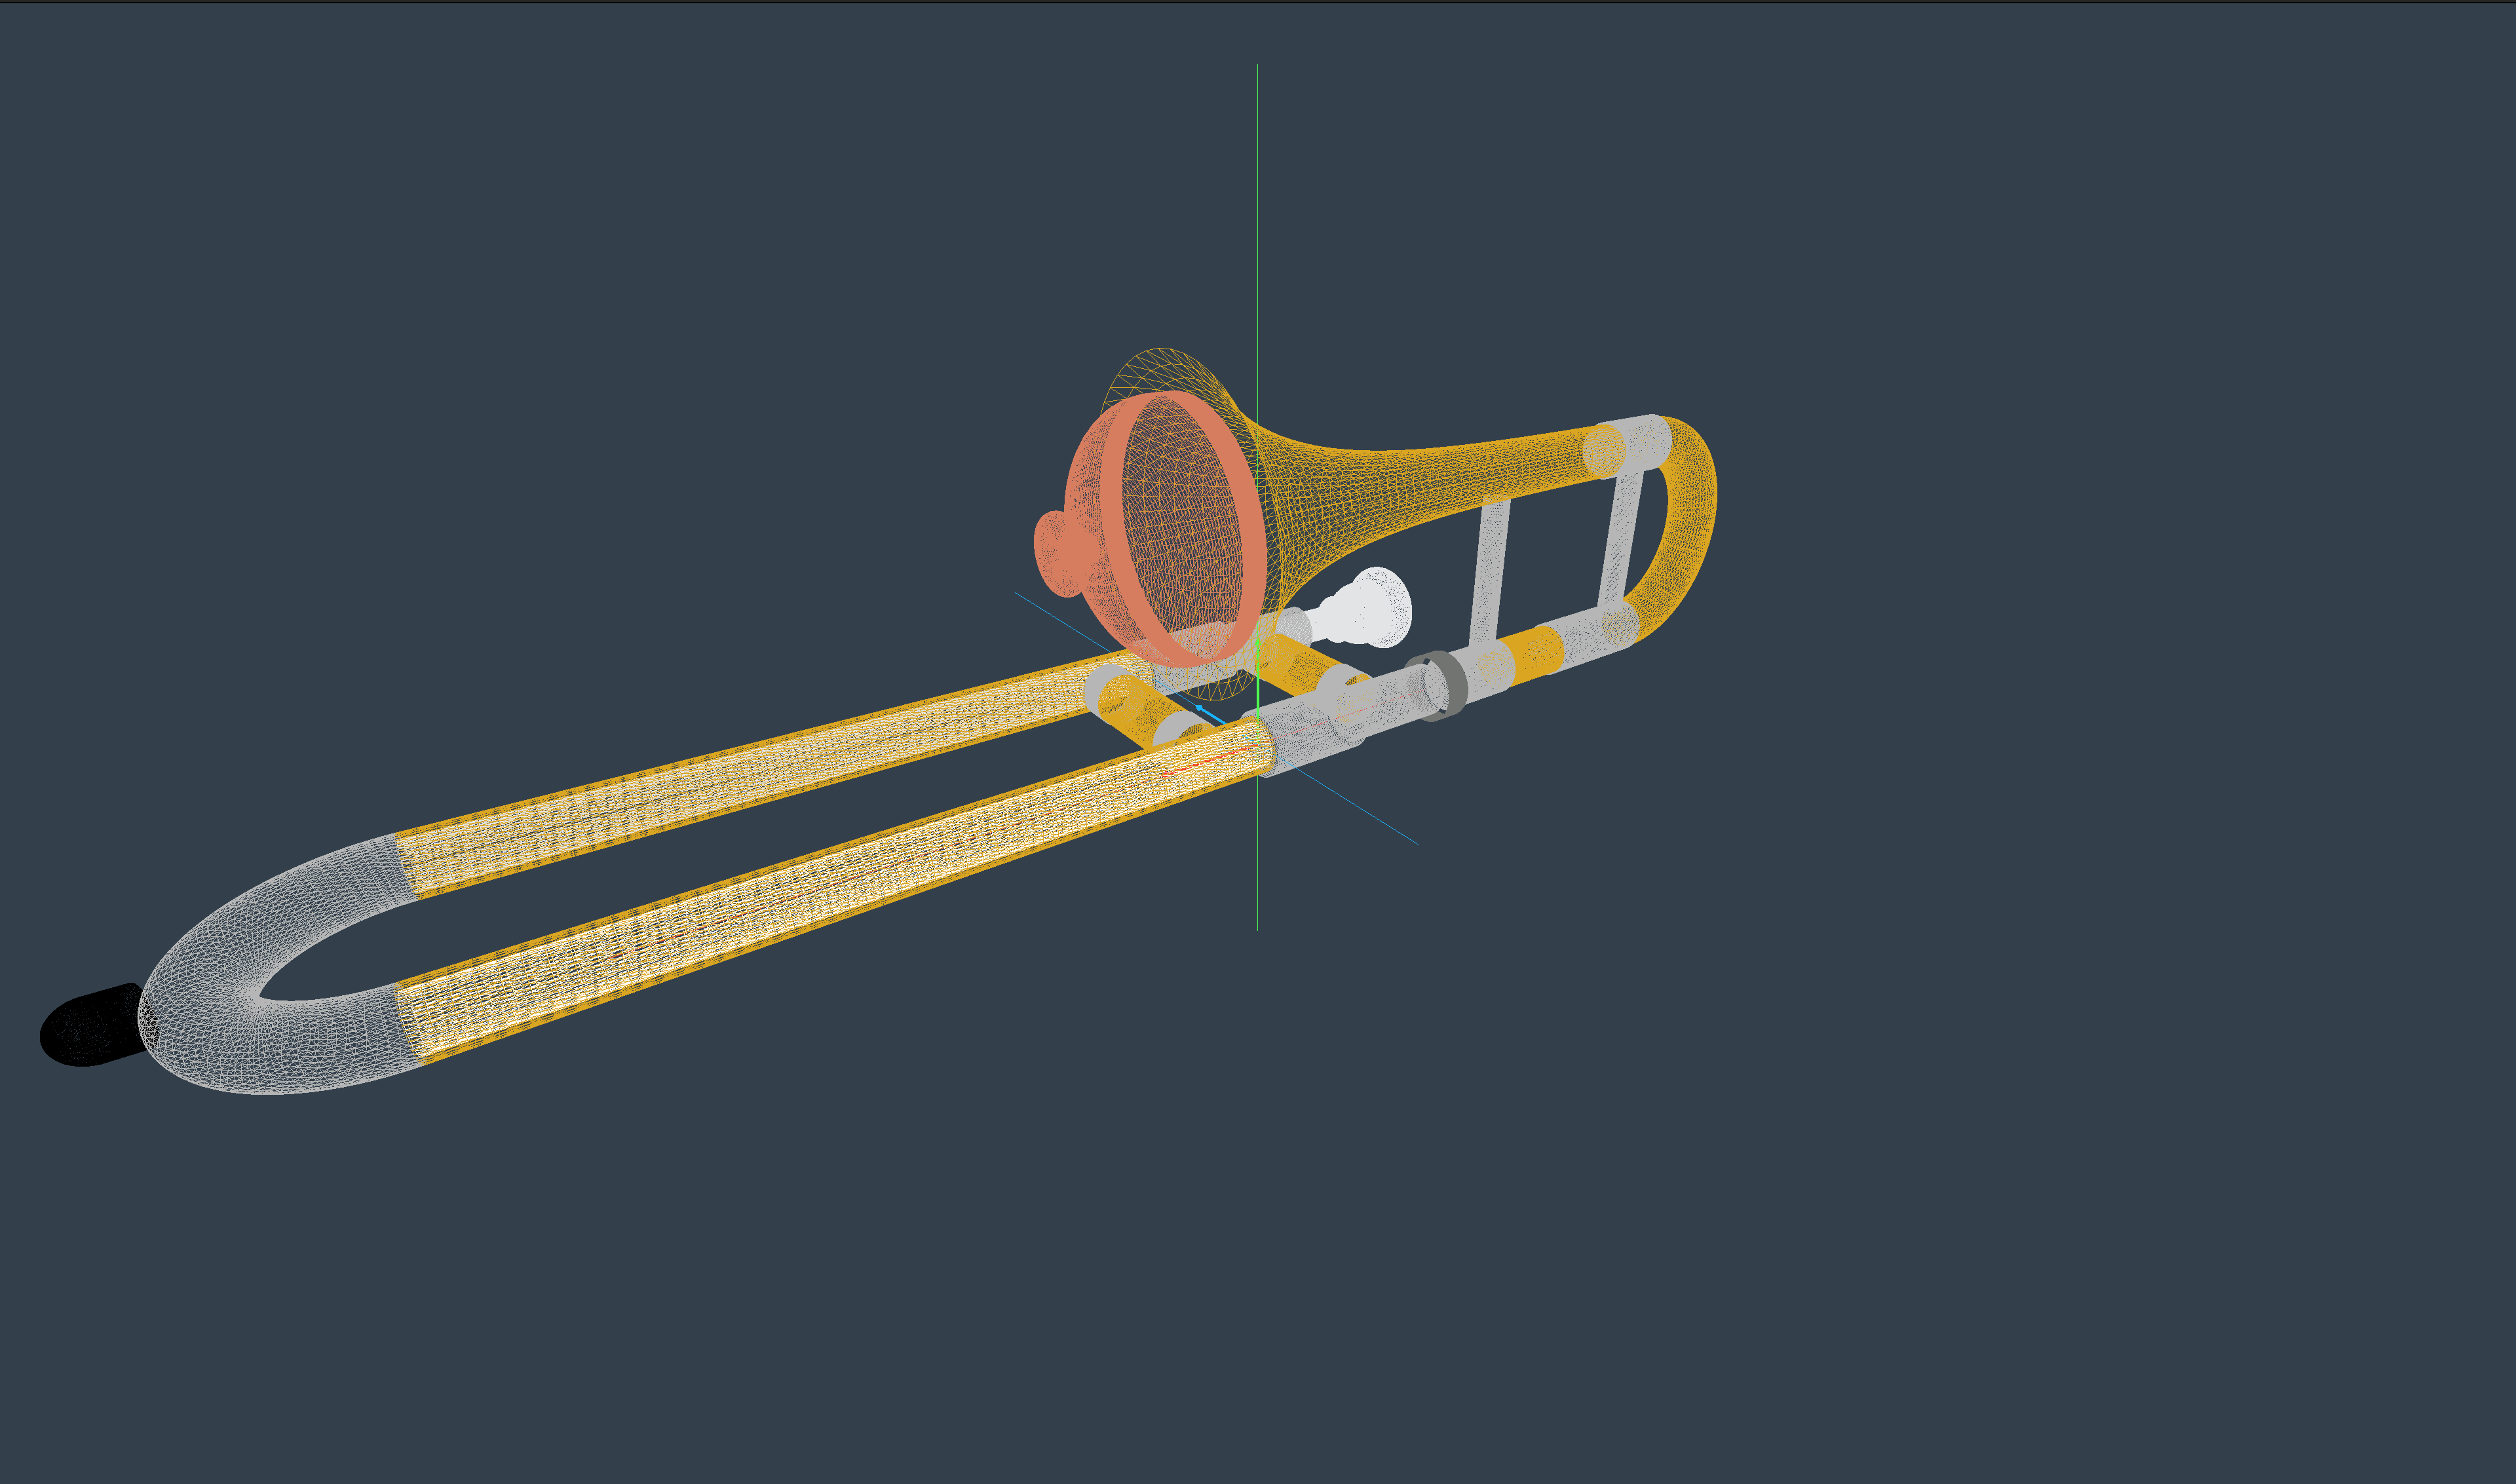
\includegraphics[width=15cm]{resources/img08.png}
\newpage
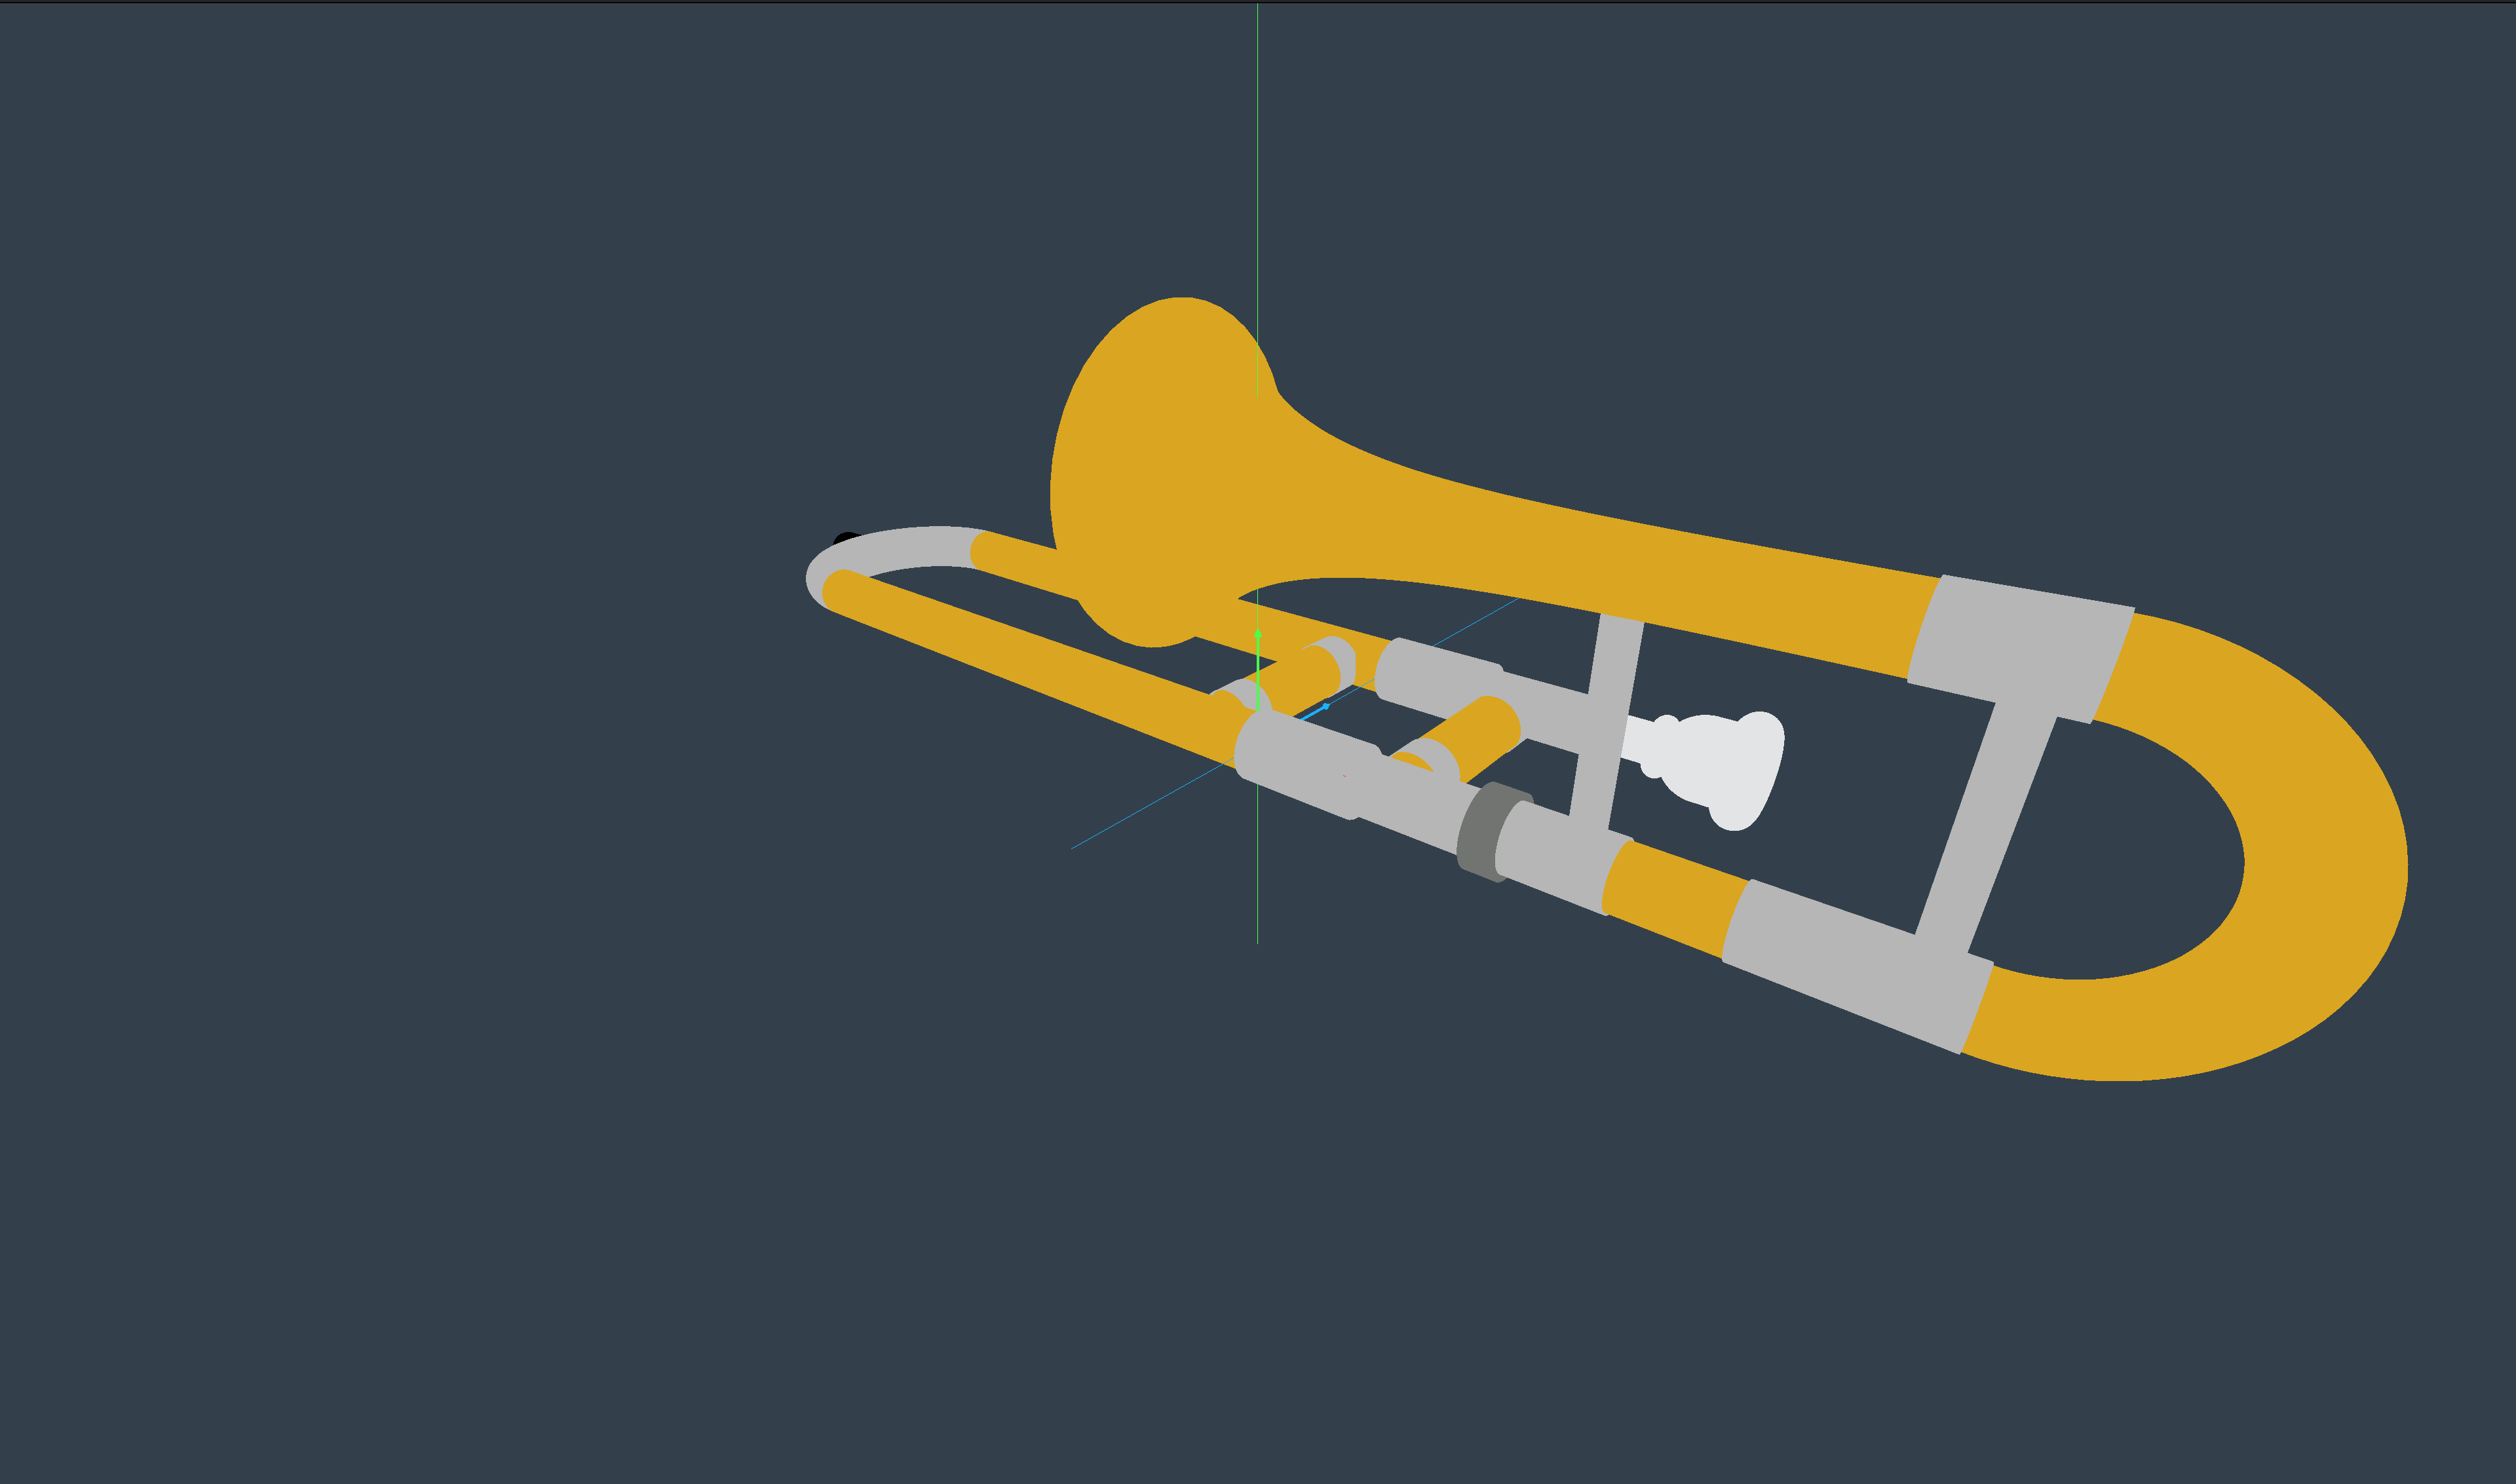
\includegraphics[width=15cm]{resources/img09.png}
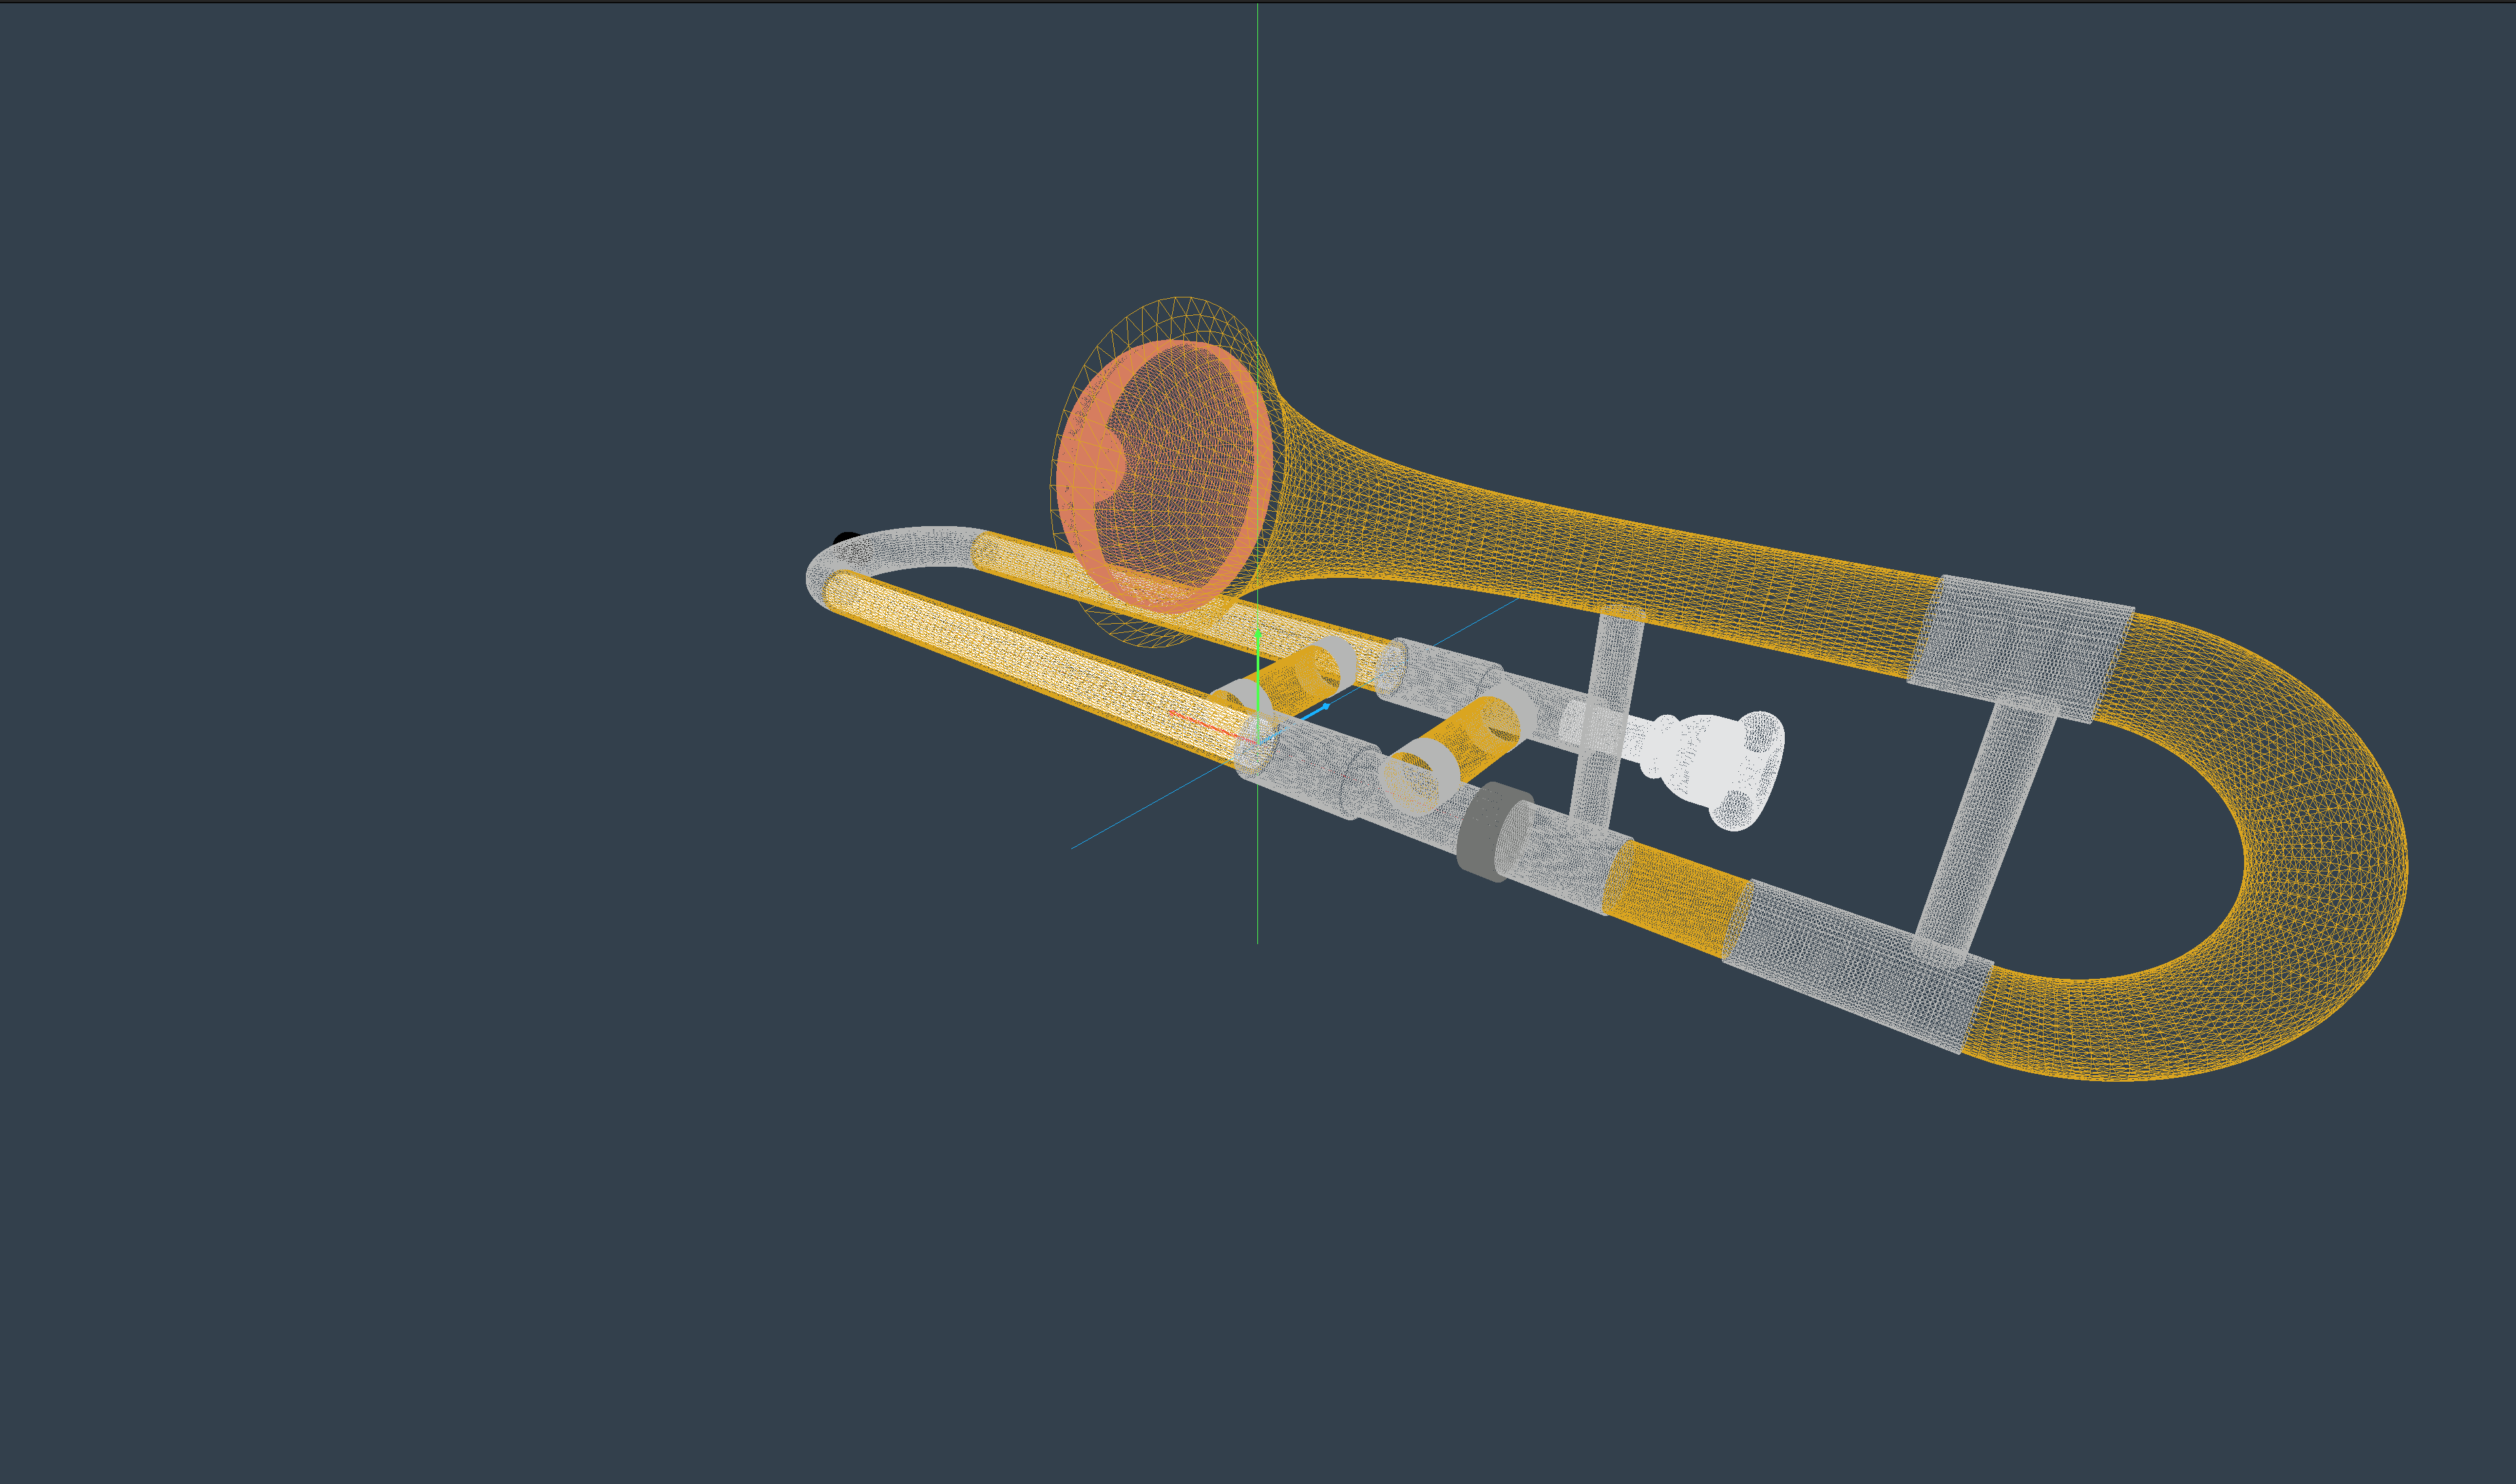
\includegraphics[width=15cm]{resources/img10.png}
\end{center}

\newpage

\section{Grafo PHIGS}

\begin{center}
	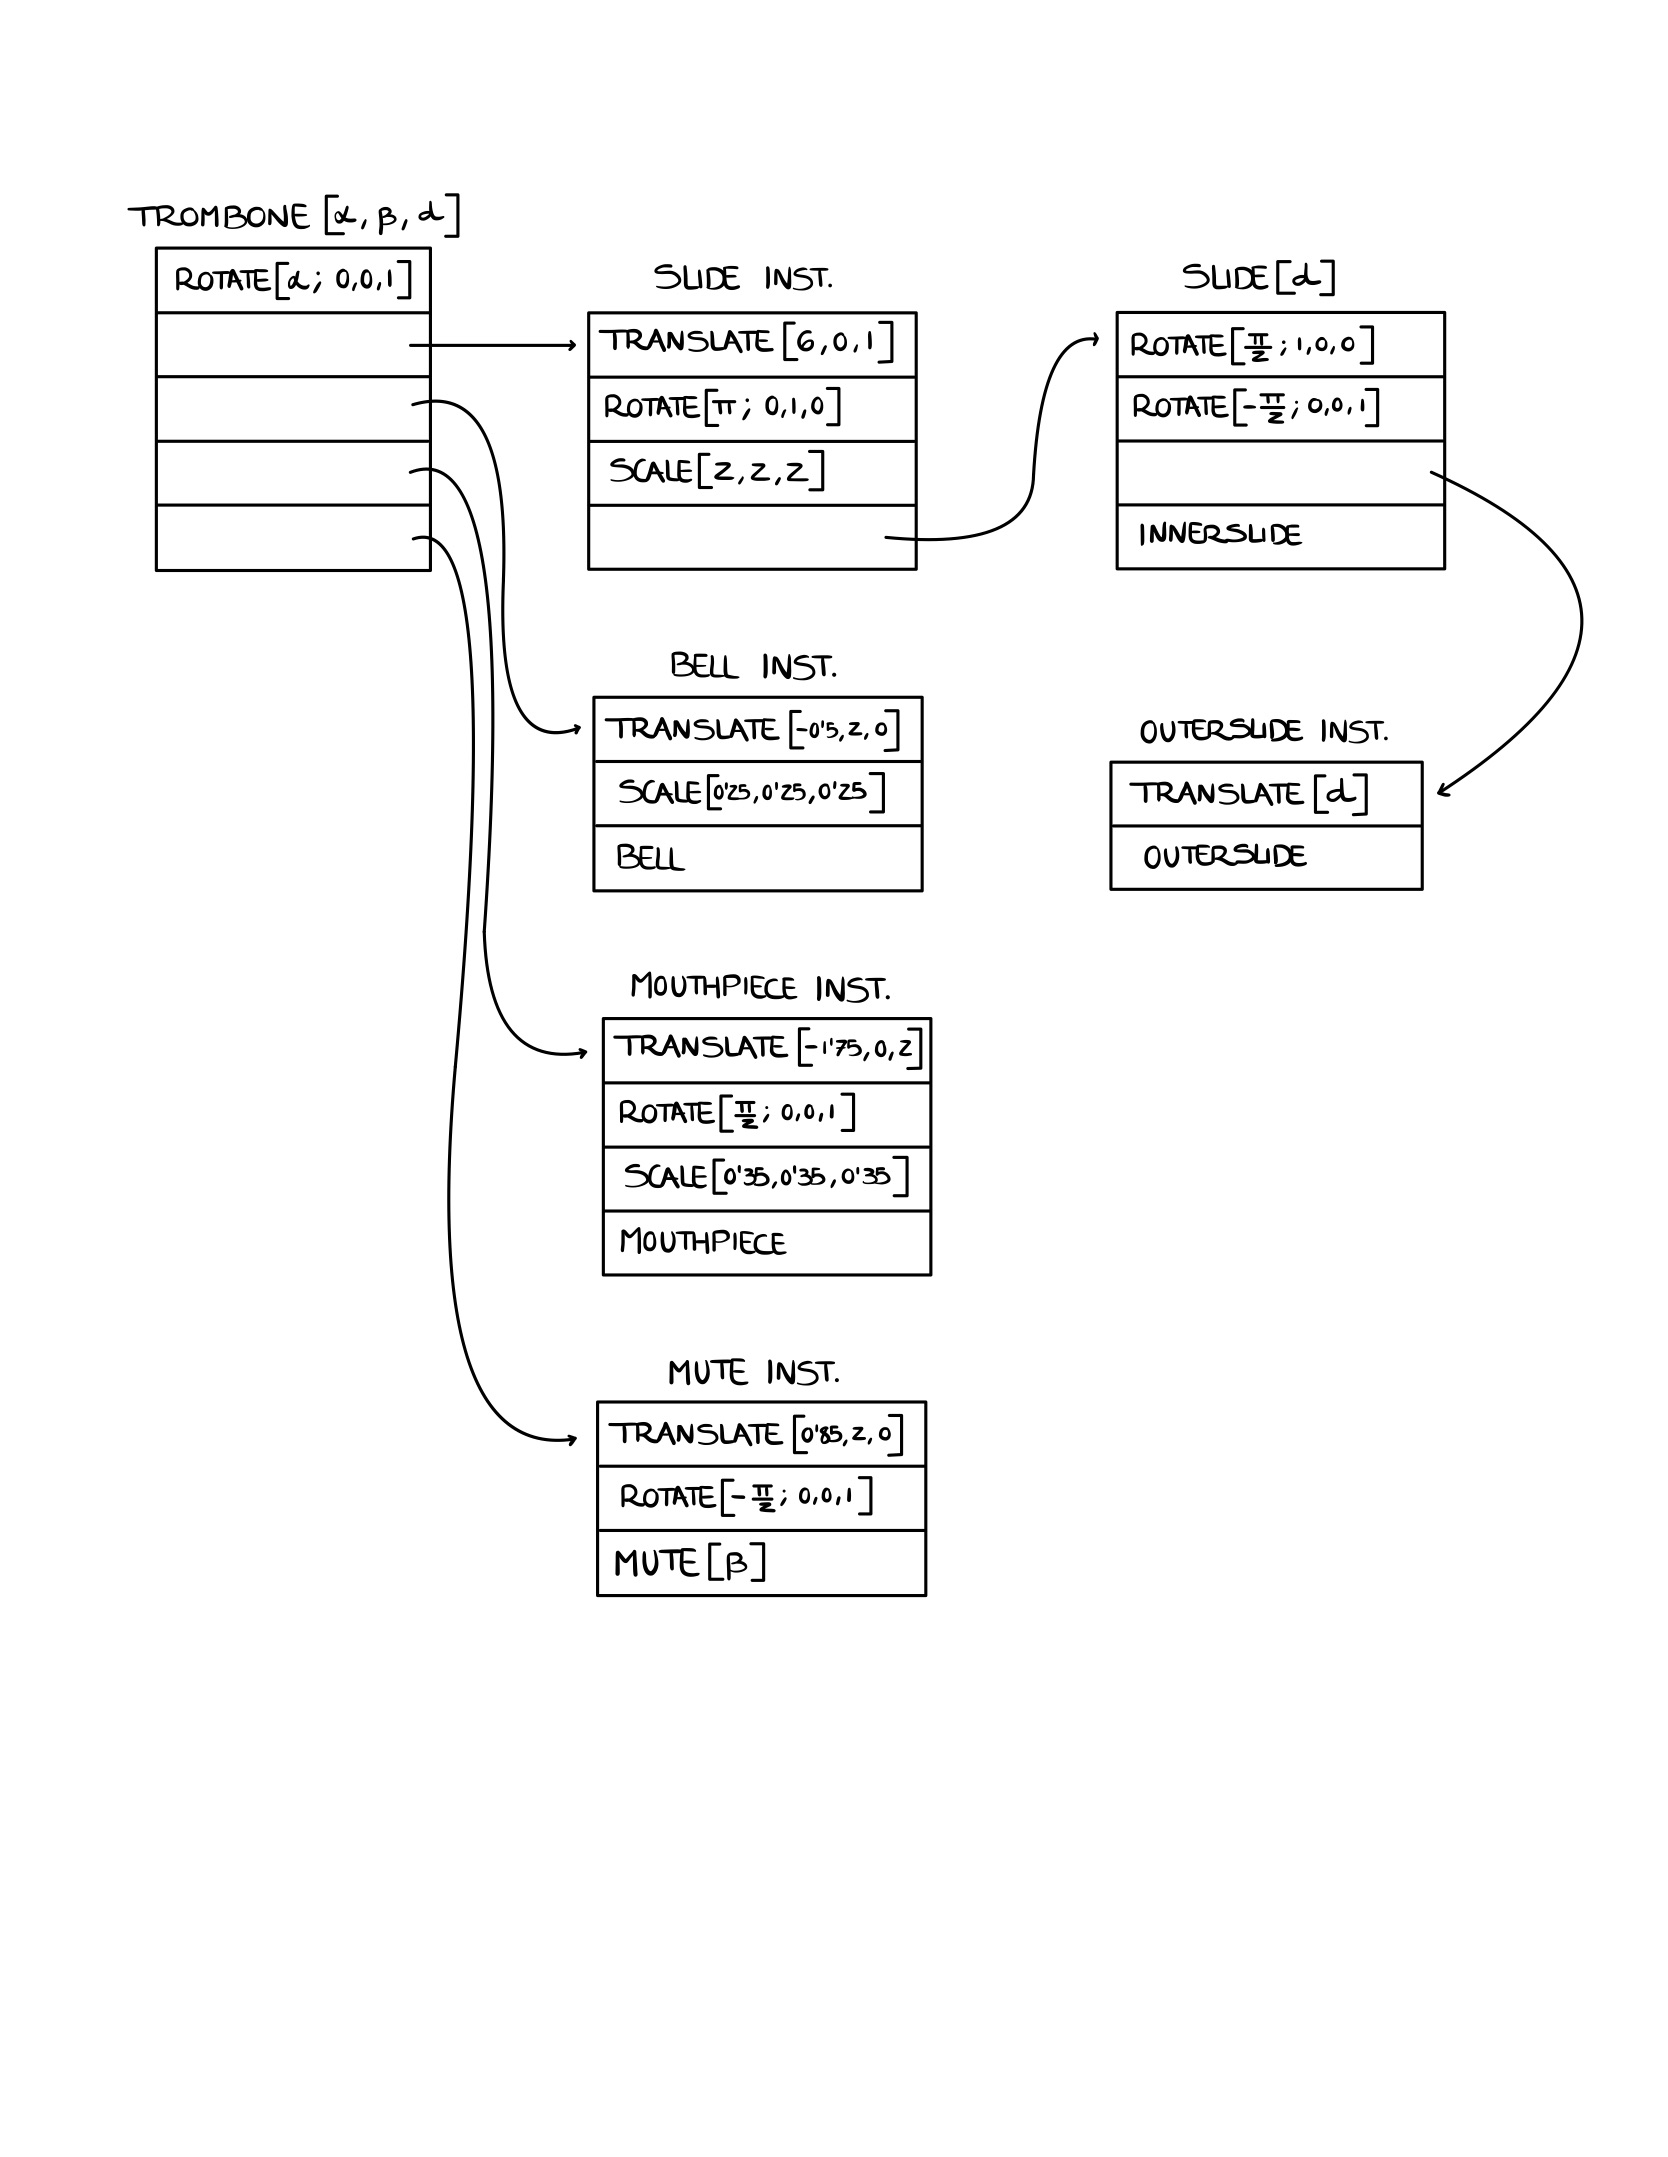
\includegraphics[width=15cm]{resources/img11.jpg}
	\newpage
	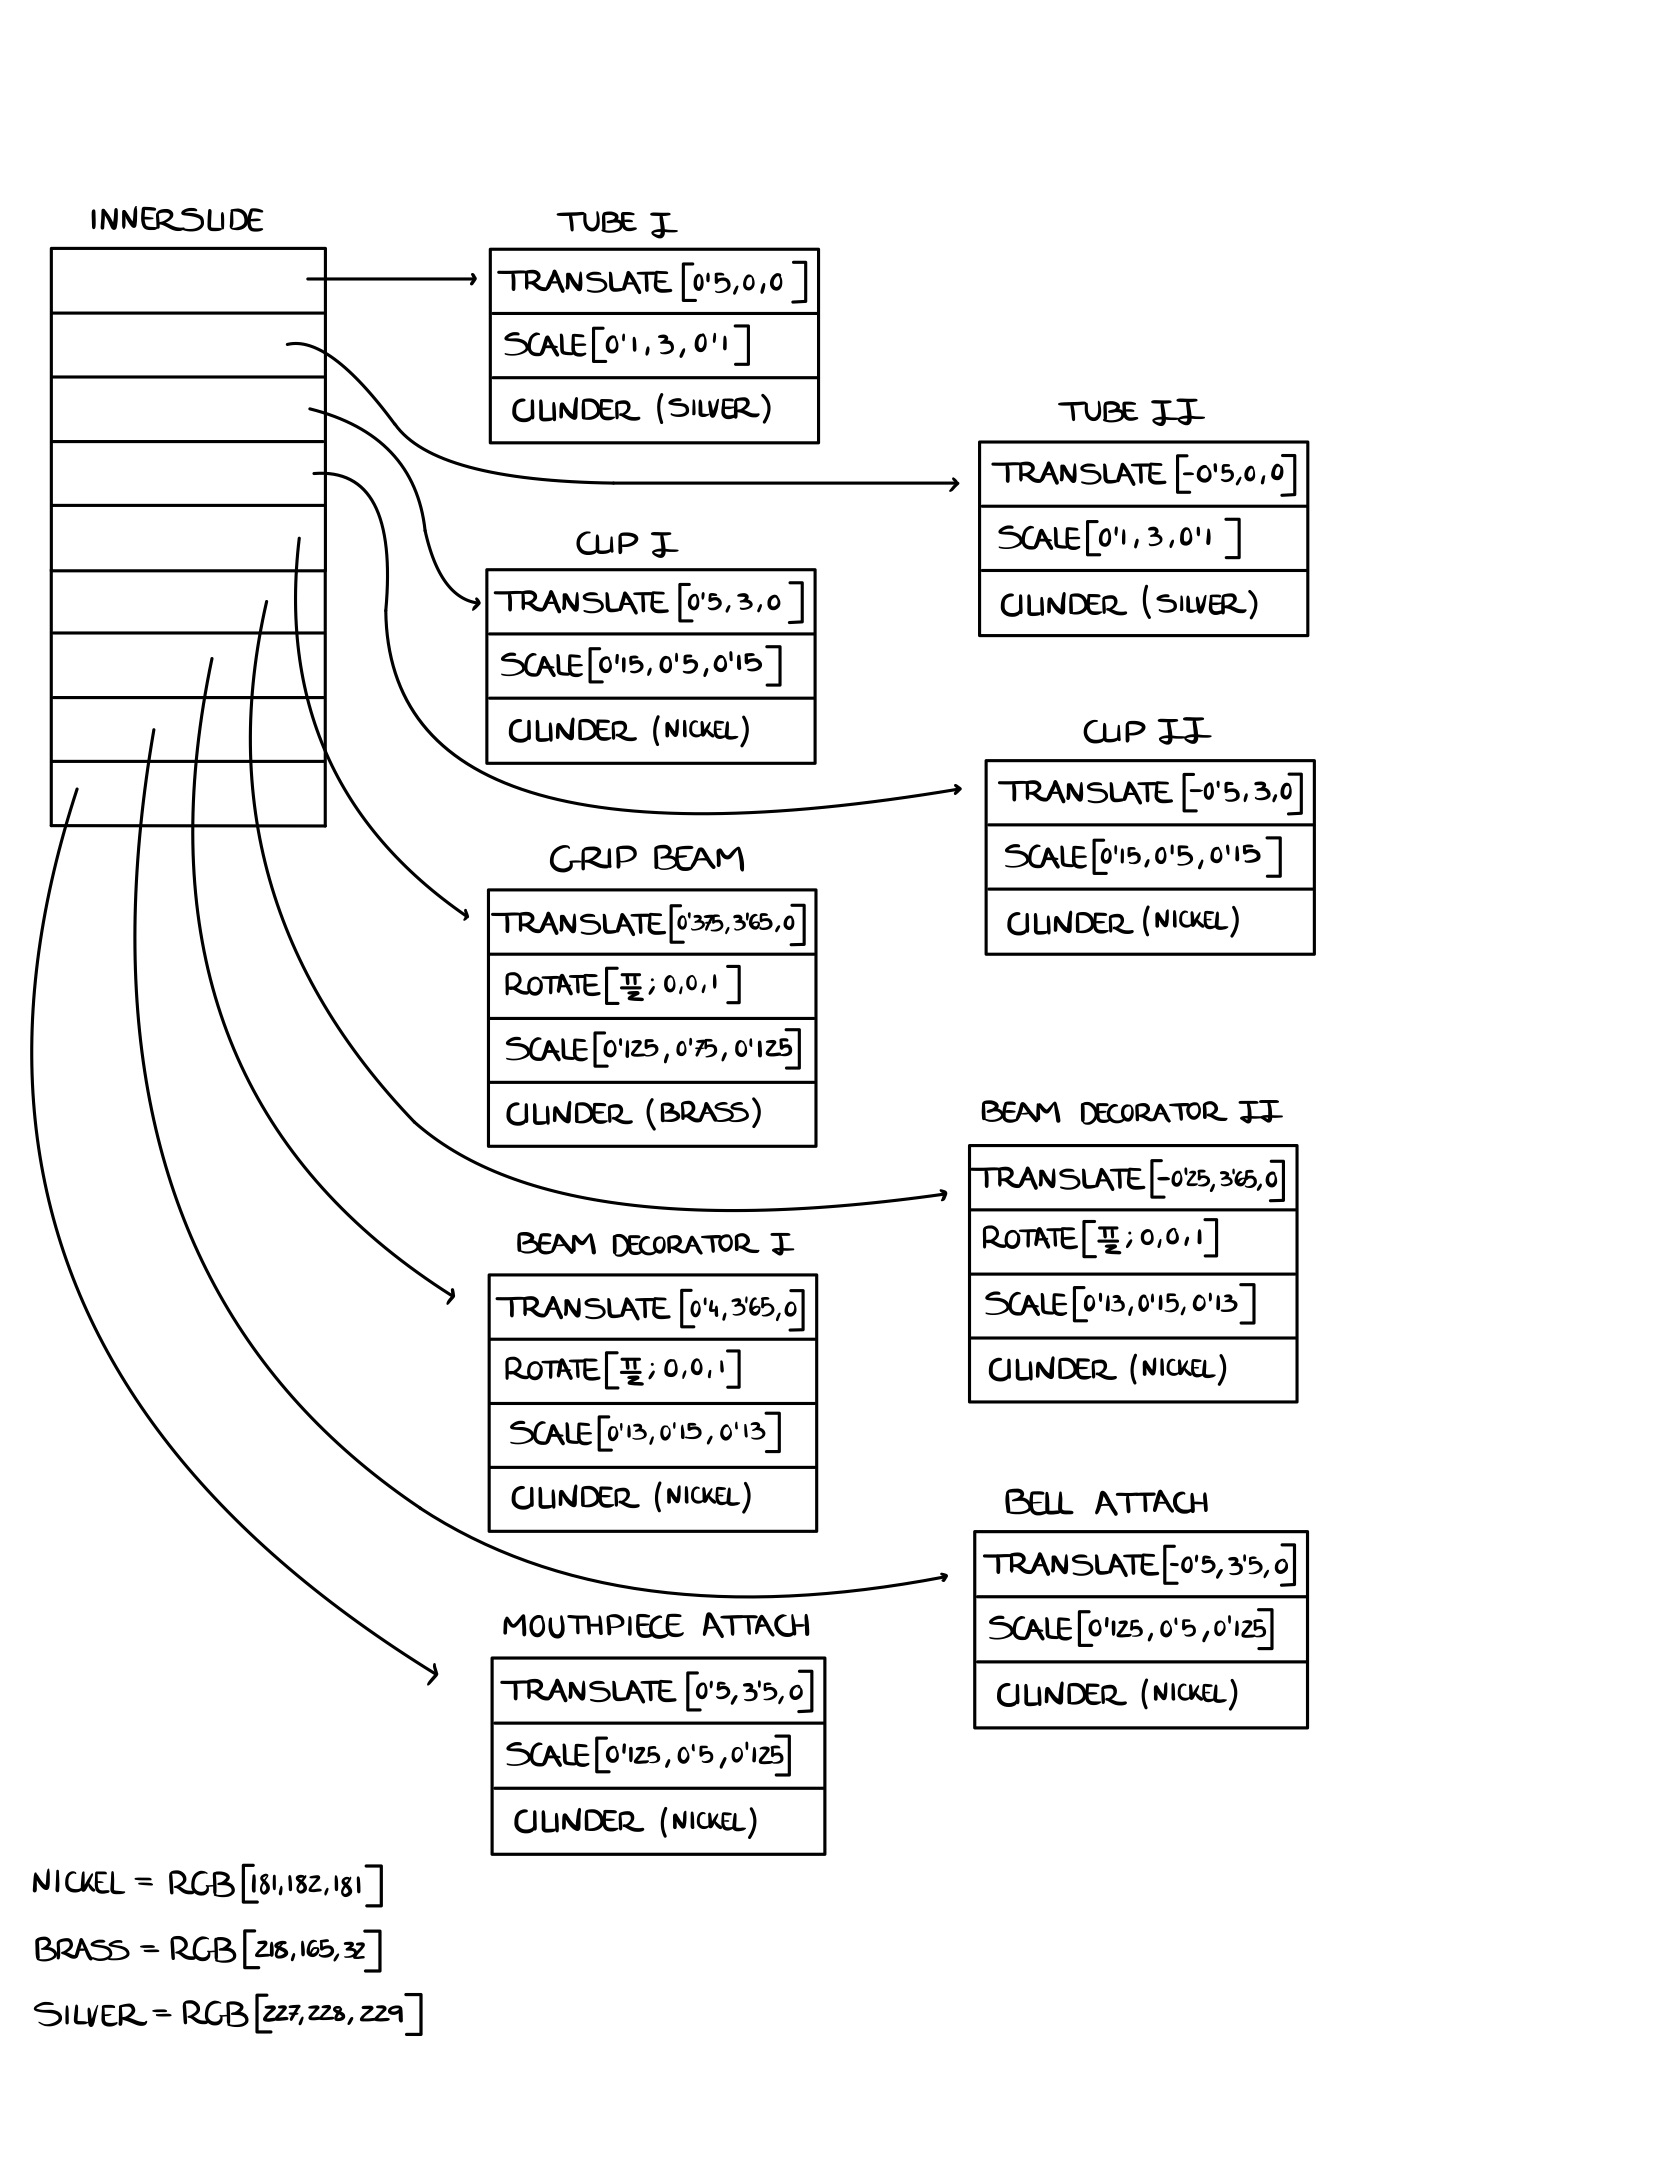
\includegraphics[width=15cm]{resources/img12.jpg}
	\newpage
	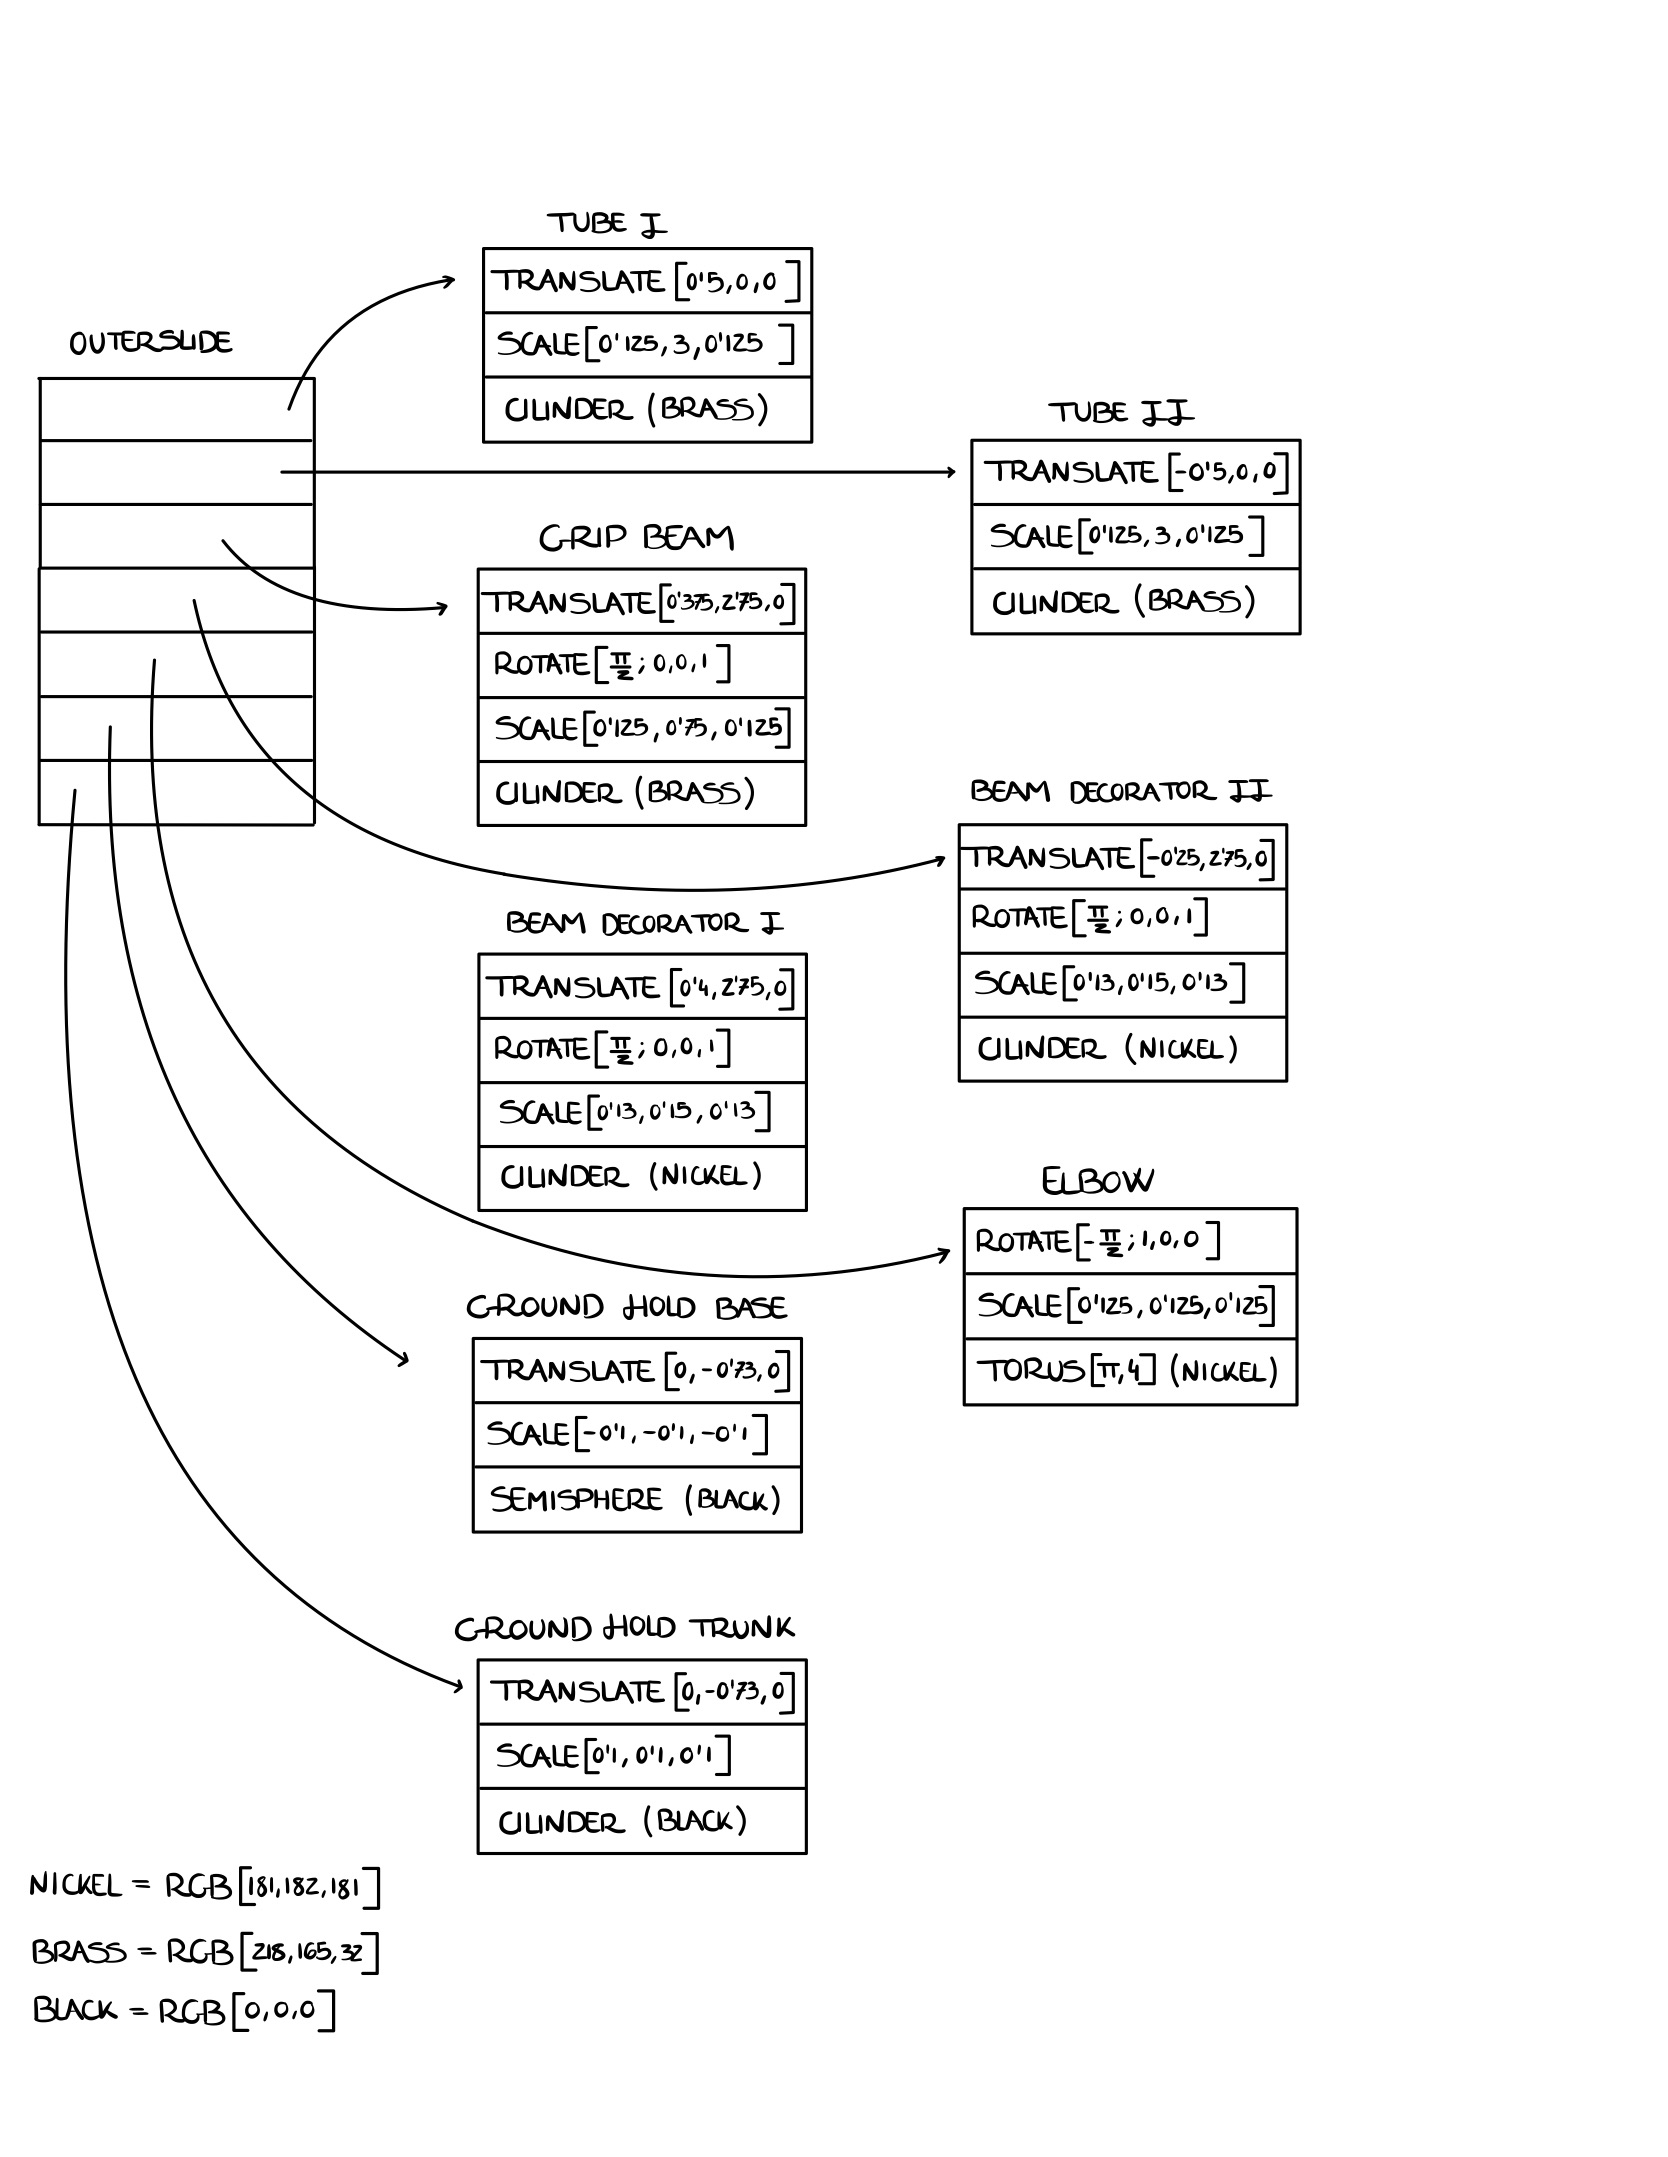
\includegraphics[width=15cm]{resources/img13.jpg}
	\newpage
	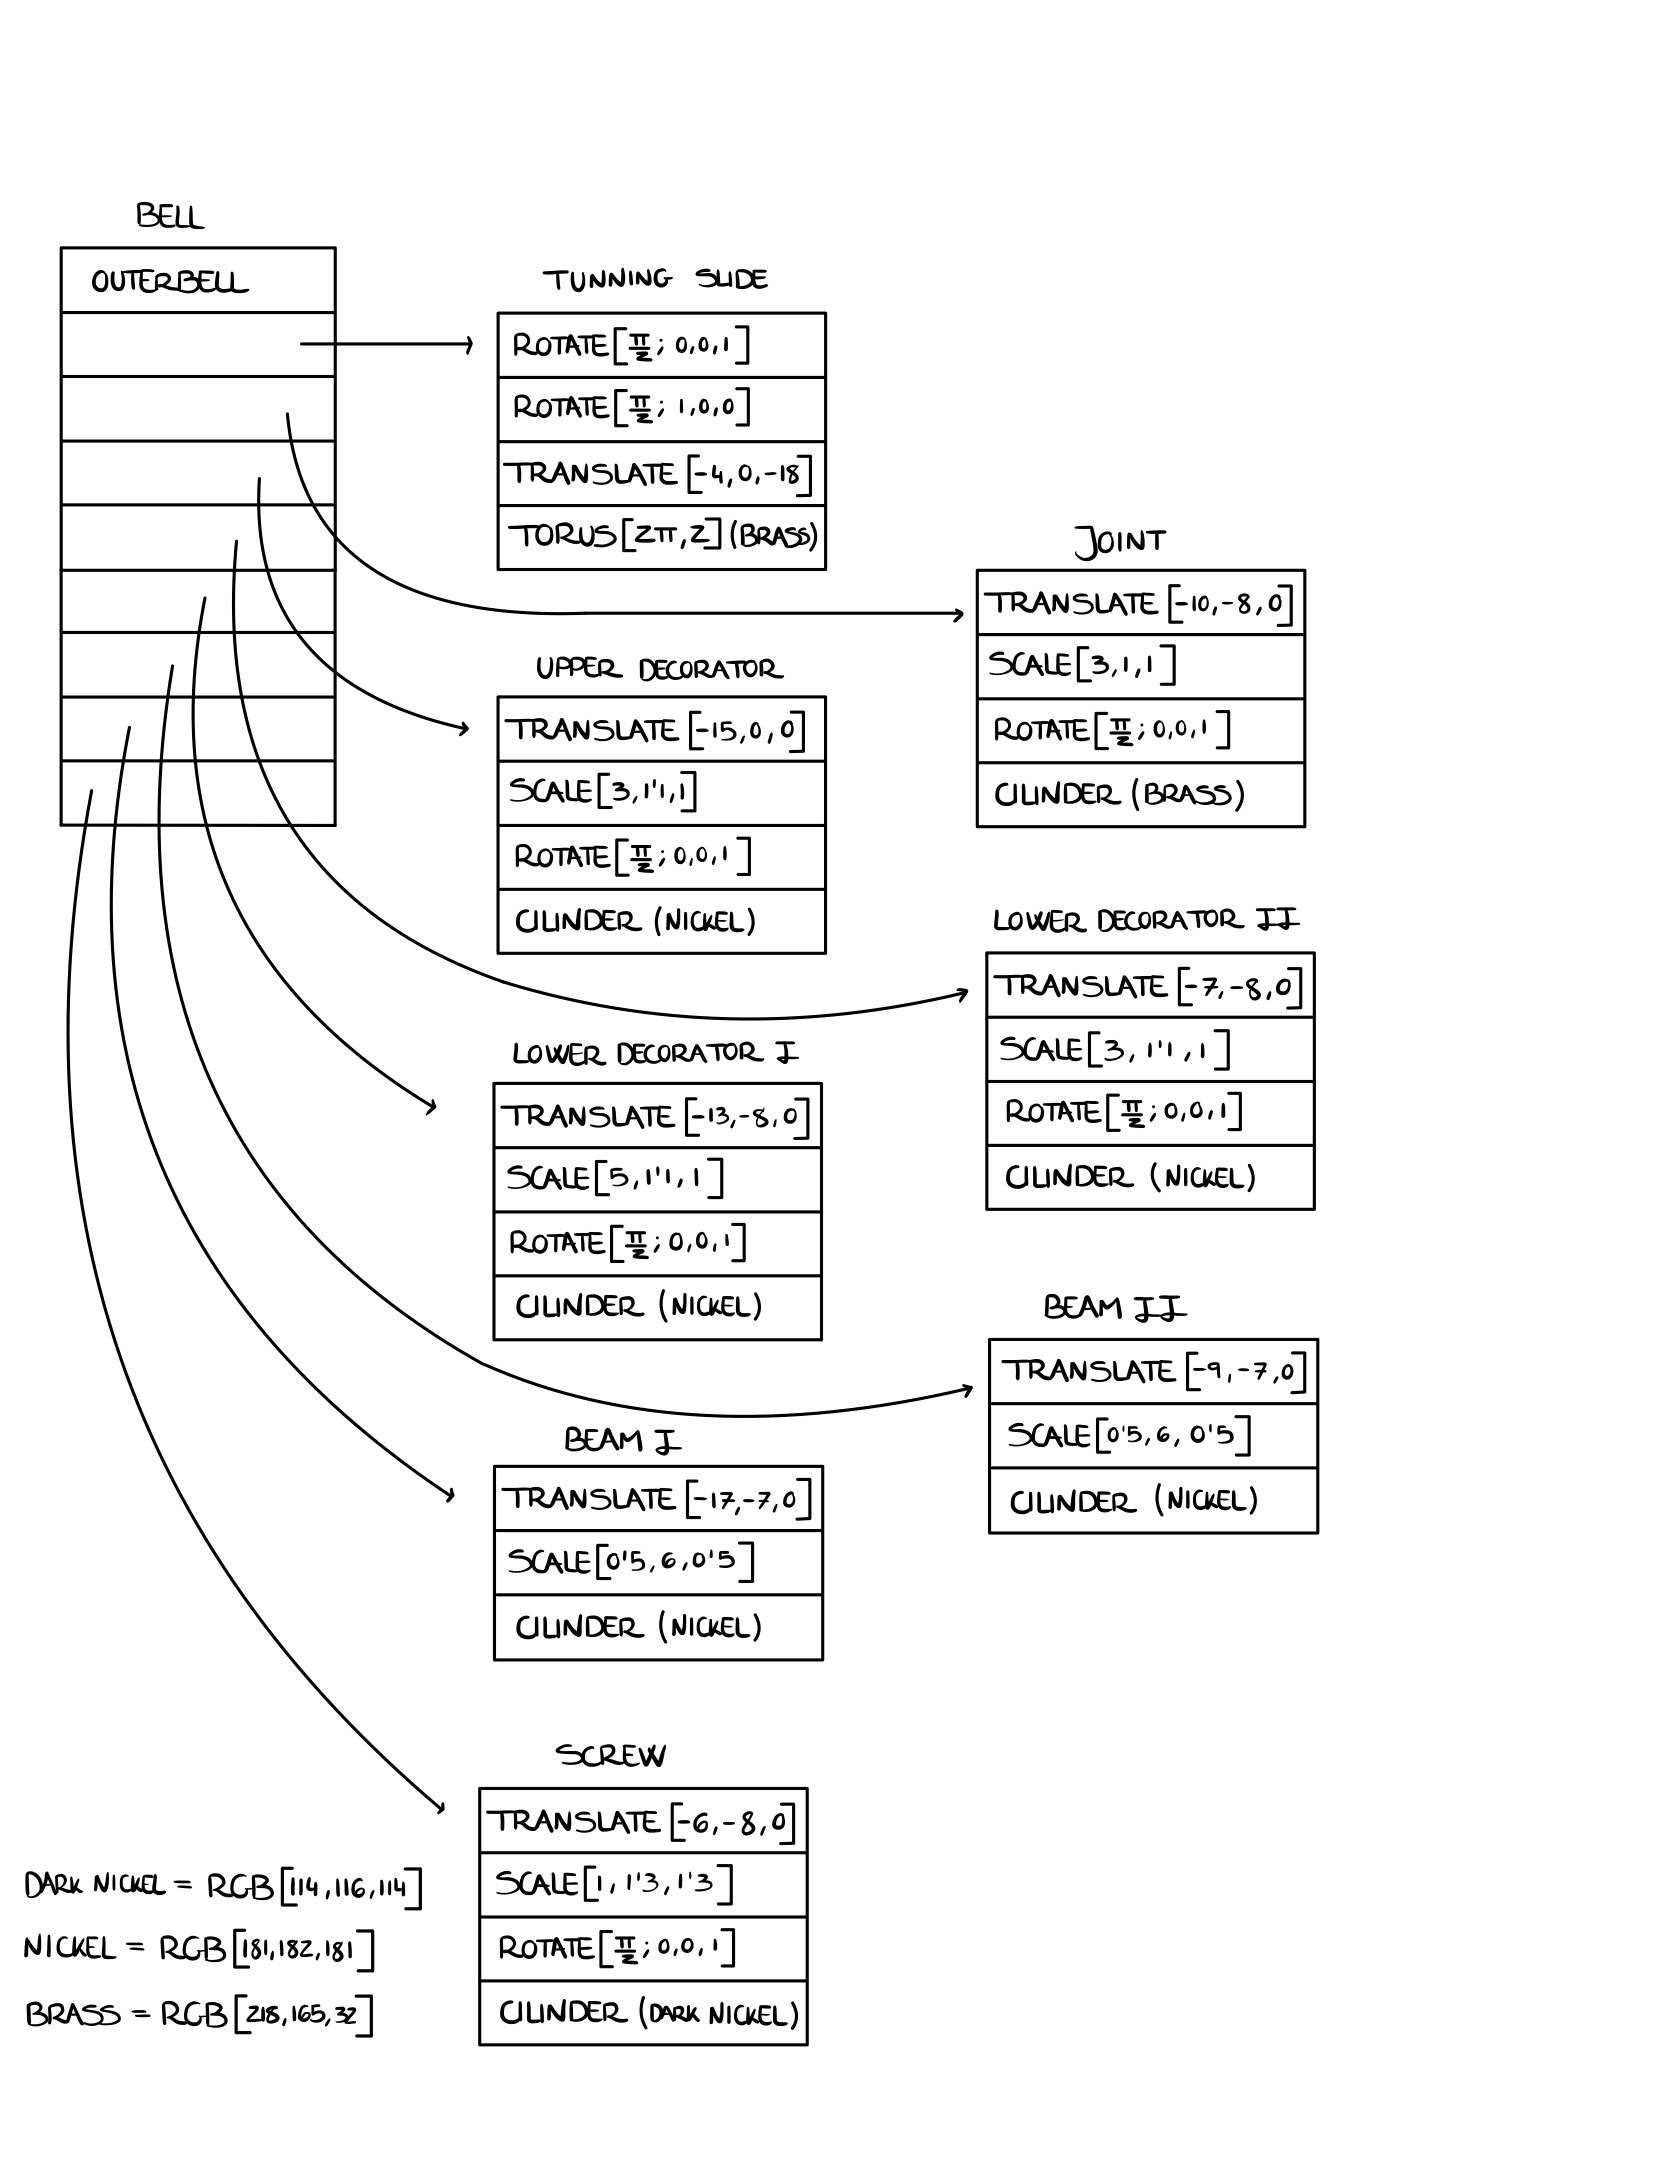
\includegraphics[width=15cm]{resources/img14.jpg}
	\newpage
	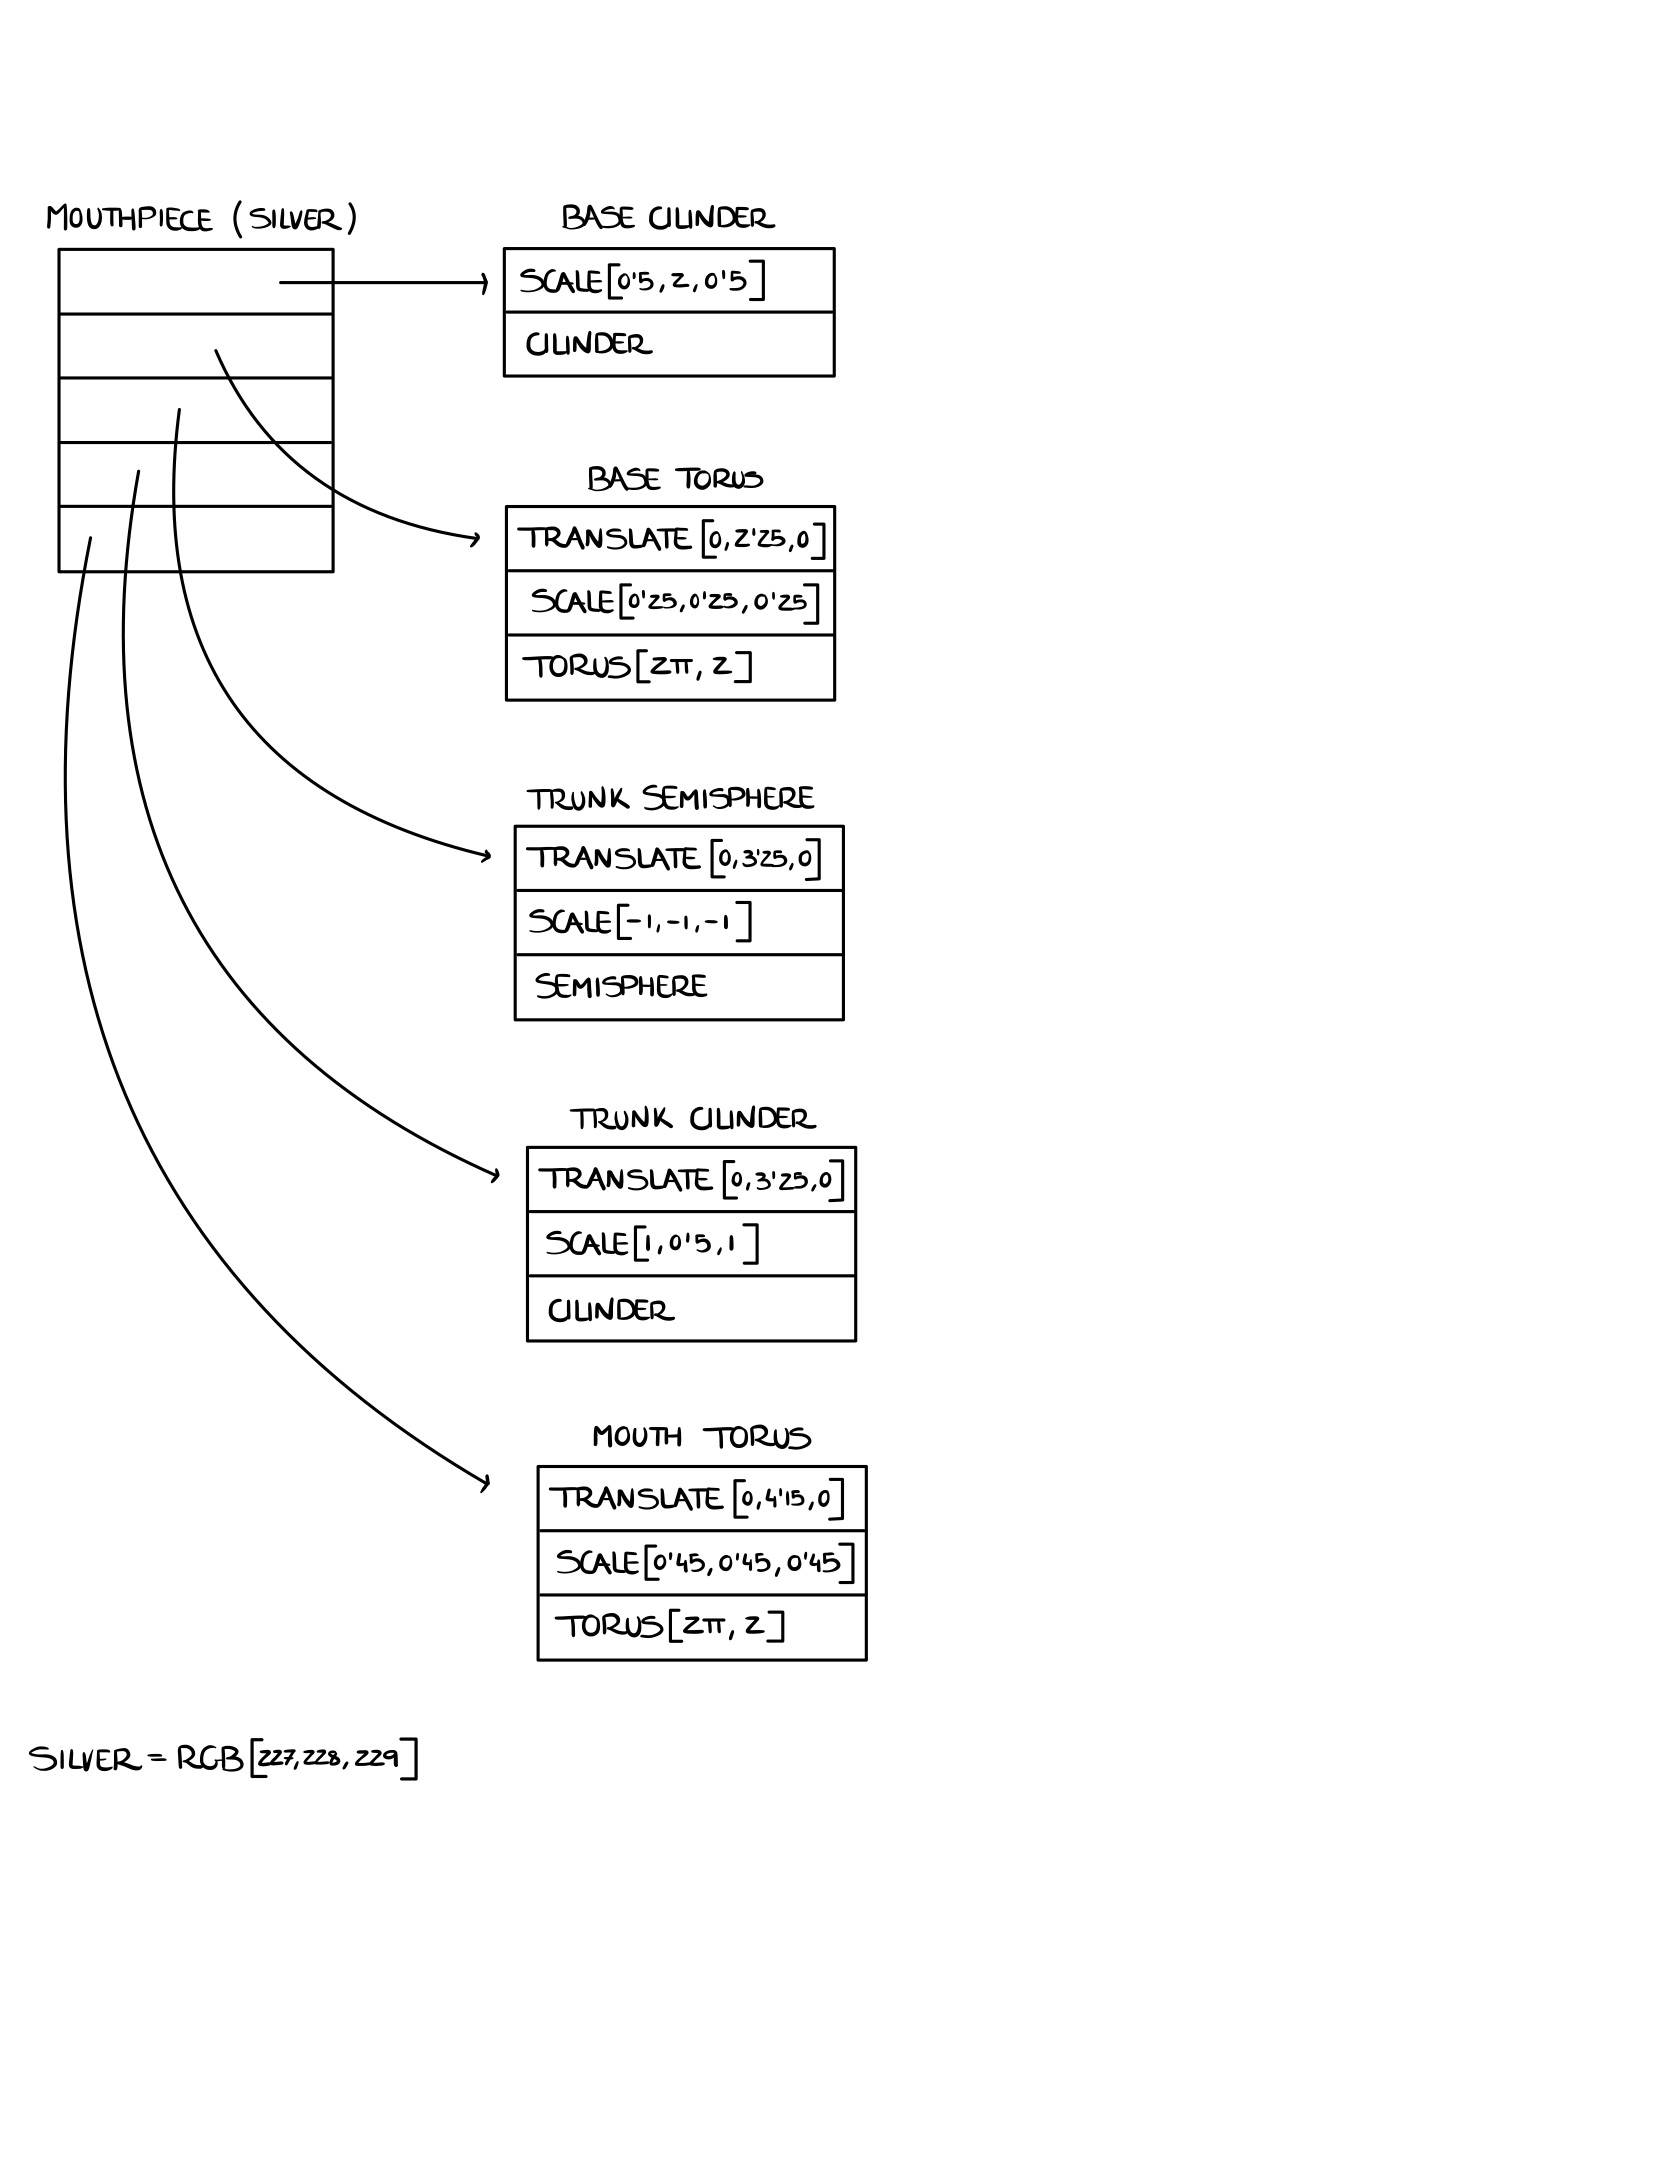
\includegraphics[width=15cm]{resources/img15.jpg}
\end{center}

\newpage

\section{Nodos del Grafo PHIGS}

\begin{enumerate}
	\item \textbf{Clase:} Cilinder
	\begin{itemize}
		\item \textbf{Archivo:} malla-revol.cpp
		\item \textbf{Rango de líneas:} 175-187
	\end{itemize}
	\item \textbf{Clase:} SemiSphere
	\begin{itemize}
		\item \textbf{Archivo:} modelo-jer.cpp
		\item \textbf{Rango de líneas:} 7-19
	\end{itemize}
	\item \textbf{Clase:} Torus
	\begin{itemize}
		\item \textbf{Archivo:} modelo-jer.cpp
		\item \textbf{Rango de líneas:} 21-32
	\end{itemize}
	\item \textbf{Clase:} OuterBell
	\begin{itemize}
		\item \textbf{Archivo:} modelo-jer.cpp
		\item \textbf{Rango de líneas:} 34-51
	\end{itemize}
	\item \textbf{Clase:} TunningSlide
	\begin{itemize}
		\item \textbf{Archivo:} modelo-jer.cpp
		\item \textbf{Rango de líneas:} 53-60
	\end{itemize}
	\item \textbf{Clase:} Bell
	\begin{itemize}
		\item \textbf{Archivo:} modelo-jer.cpp
		\item \textbf{Rango de líneas:} 62-120
	\end{itemize}
	\item \textbf{Objeto:} joint
	\begin{itemize}
		\item \textbf{Instanciado en Clase:} Bell
		\item \textbf{Color:} (218, 165, 32)
		\item \textbf{Rango de líneas:} 64-69
	\end{itemize}
	\item \textbf{Objeto:} upperdecorator
	\begin{itemize}
		\item \textbf{Instanciado en Clase:} Bell
		\item \textbf{Color:} (181, 182, 181)
		\item \textbf{Rango de líneas:} 71-76
	\end{itemize}
	\item \textbf{Objeto:} lowerdecorator1 
	\begin{itemize}
		\item \textbf{Instanciado en Clase:} Bell
		\item \textbf{Color:} (181, 182, 181)
		\item \textbf{Rango de líneas:} 78-83
	\end{itemize}
	\item \textbf{Objeto:} lowerdecorator2
	\begin{itemize}
		\item \textbf{Instanciado en Clase:} Bell
		\item \textbf{Color:} (181, 182, 181)
		\item \textbf{Rango de líneas:} 85-90
	\end{itemize}
	\item \textbf{Objeto:} beam1 
	\begin{itemize}
		\item \textbf{Instanciado en Clase:} Bell
		\item \textbf{Color:} (181, 182, 181)
		\item \textbf{Rango de líneas:} 92-96
	\end{itemize}
	\item \textbf{Objeto:} beam2
	\begin{itemize}
		\item \textbf{Instanciado en Clase:} Bell
		\item \textbf{Color:} (181, 182, 181)
		\item \textbf{Rango de líneas:} 98-102
	\end{itemize}
	\item \textbf{Objeto:} screw
	\begin{itemize}
		\item \textbf{Instanciado en Clase:} Bell
		\item \textbf{Color:} (114, 116, 114)
		\item \textbf{Rango de líneas:} 104-109
	\end{itemize}
	\item \textbf{Clase:} InnerSlide
	\begin{itemize}
		\item \textbf{Archivo:} modelo-jer.cpp
		\item \textbf{Rango de líneas:} 122-190
	\end{itemize}
	\item \textbf{Objeto:} tube1
	\begin{itemize}
		\item \textbf{Instanciado en Clase:} InnerSlide
		\item \textbf{Color:} (227, 228, 229)
		\item \textbf{Rango de líneas:} 124-128
	\end{itemize}
	\item \textbf{Objeto:} tube2
	\begin{itemize}
		\item \textbf{Instanciado en Clase:} InnerSlide
		\item \textbf{Color:} (227, 228, 229)
		\item \textbf{Rango de líneas:} 130-134
	\end{itemize}
	\item \textbf{Objeto:} clip1
	\begin{itemize}
		\item \textbf{Instanciado en Clase:} InnerSlide
		\item \textbf{Color:} (181, 182, 181)
		\item \textbf{Rango de líneas:} 136-140
	\end{itemize}
	\item \textbf{Objeto:} clip2
	\begin{itemize}
		\item \textbf{Instanciado en Clase:} InnerSlide
		\item \textbf{Color:} (181, 182, 181)
		\item \textbf{Rango de líneas:} 142-146
	\end{itemize}
	\item \textbf{Objeto:} beamdecorator1
	\begin{itemize}
		\item \textbf{Instanciado en Clase:} InnerSlide
		\item \textbf{Color:} (181, 182, 181)
		\item \textbf{Rango de líneas:} 148-153
	\end{itemize}
	\item \textbf{Objeto:} beamdecorator2
	\begin{itemize}
		\item \textbf{Instanciado en Clase:} InnerSlide
		\item \textbf{Color:} (181, 182, 181)
		\item \textbf{Rango de líneas:} 155-160
	\end{itemize}
	\item \textbf{Objeto:} gripbeam
	\begin{itemize}
		\item \textbf{Instanciado en Clase:} InnerSlide
		\item \textbf{Color:} (218, 165, 32)
		\item \textbf{Rango de líneas:} 162-167
	\end{itemize}
	\item \textbf{Objeto:} mouthpieceattach
	\begin{itemize}
		\item \textbf{Instanciado en Clase:} InnerSlide
		\item \textbf{Color:} (181, 182, 181)
		\item \textbf{Rango de líneas:} 169-173
	\end{itemize}
	\item \textbf{Objeto:} bellattach
	\begin{itemize}
		\item \textbf{Instanciado en Clase:} InnerSlide
		\item \textbf{Color:} (181, 182, 181)
		\item \textbf{Rango de líneas:} 175-179
	\end{itemize}
	\item \textbf{Clase:} OuterSlide 
	\begin{itemize}
		\item \textbf{Archivo:} modelo-jer.cpp
		\item \textbf{Rango de líneas:} 192-253
	\end{itemize}
	\item \textbf{Objeto:} tube1
	\begin{itemize}
		\item \textbf{Instanciado en Clase:} OuterSlide
		\item \textbf{Color:} (218, 165, 32)
		\item \textbf{Rango de líneas:} 194-198
	\end{itemize}
	\item \textbf{Objeto:} tube2
	\begin{itemize}
		\item \textbf{Instanciado en Clase:} OuterSlide
		\item \textbf{Color:} (218, 165, 32)
		\item \textbf{Rango de líneas:} 200-204
	\end{itemize}
	\item \textbf{Objeto:} beamdecorator1
	\begin{itemize}
		\item \textbf{Instanciado en Clase:} OuterSlide
		\item \textbf{Color:} (181, 182, 181)
		\item \textbf{Rango de líneas:} 206-211
	\end{itemize}
	\item \textbf{Objeto:} beamdecorator2
	\begin{itemize}
		\item \textbf{Instanciado en Clase:} OuterSlide
		\item \textbf{Color:} (181, 182, 181)
		\item \textbf{Rango de líneas:} 213-218
	\end{itemize}
	\item \textbf{Objeto:} gripbeam 
	\begin{itemize}
		\item \textbf{Instanciado en Clase:} OuterSlide
		\item \textbf{Color:} (218, 165, 32)
		\item \textbf{Rango de líneas:} 220-225
	\end{itemize}
	\item \textbf{Objeto:} elbow
	\begin{itemize}
		\item \textbf{Instanciado en Clase:} OuterSlide
		\item \textbf{Color:} (181, 182, 181)
		\item \textbf{Rango de líneas:} 227-231
	\end{itemize}
	\item \textbf{Objeto:} groundholdtrunk
	\begin{itemize}
		\item \textbf{Instanciado en Clase:} OuterSlide
		\item \textbf{Color:} (0, 0, 0)
		\item \textbf{Rango de líneas:} 233-237
	\end{itemize}
	\item \textbf{Objeto:} groundholdbase 
	\begin{itemize}
		\item \textbf{Instanciado en Clase:} OuterSlide
		\item \textbf{Color:} (0, 0, 0)
		\item \textbf{Rango de líneas:} 239-243
	\end{itemize}
	\item \textbf{Clase:} Slide
	\begin{itemize}
		\item \textbf{Grados de Libertad:} slidemovement
		\item \textbf{Archivo:} modelo-jer.cpp
		\item \textbf{Rango de líneas:} 255-270
	\end{itemize}
	\item \textbf{Clase:} Mouthpiece
	\begin{itemize}
		\item \textbf{Archivo:} modelo-jer.cpp
		\item \textbf{Rango de líneas:} 290-322
	\end{itemize}
	\item \textbf{Objeto:} basecilinder 
	\begin{itemize}
		\item \textbf{Instanciado en Clase:} Mouthpiece
		\item \textbf{Color:} (227, 229, 229)
		\item \textbf{Rango de líneas:} 292-294
	\end{itemize}
	\item \textbf{Objeto:} basetorus
	\begin{itemize}
		\item \textbf{Instanciado en Clase:} Mouthpiece
		\item \textbf{Color:} (227, 229, 229)
		\item \textbf{Rango de líneas:} 296-299
	\end{itemize}
	\item \textbf{Objeto:} trunksemisphere
	\begin{itemize}
		\item \textbf{Instanciado en Clase:} Mouthpiece
		\item \textbf{Color:} (227, 229, 229)
		\item \textbf{Rango de líneas:} 301-304
	\end{itemize}
	\item \textbf{Objeto:} trunkcilinder 
	\begin{itemize}
		\item \textbf{Instanciado en Clase:} Mouthpiece
		\item \textbf{Color:} (227, 229, 229)
		\item \textbf{Rango de líneas:} 306-309
	\end{itemize}
	\item \textbf{Objeto:} mouthtorus
	\begin{itemize}
		\item \textbf{Instanciado en Clase:} Mouthpiece
		\item \textbf{Color:} (227, 229, 229)
		\item \textbf{Rango de líneas:} 311-314
	\end{itemize}
	\item \textbf{Clase:} Mute
	\begin{itemize}
		\item \textbf{Grados de Libertad:} mutemovement
		\item \textbf{Archivo:} modelo-jer.cpp
		\item \textbf{Rango de líneas:} 324-353
	\end{itemize}
	\item \textbf{Objeto:} cup
	\begin{itemize}
		\item \textbf{Instanciado en Clase:} Mute
		\item \textbf{Color:} (214, 125, 95)
		\item \textbf{Rango de líneas:} 326-328
	\end{itemize}
	\item \textbf{Objeto:} base
	\begin{itemize}
		\item \textbf{Instanciado en Clase:} Mute
		\item \textbf{Color:} (214, 125, 95)
		\item \textbf{Rango de líneas:} 330-333
	\end{itemize}
	\item \textbf{Objeto:} gripend
	\begin{itemize}
		\item \textbf{Instanciado en Clase:} Mute
		\item \textbf{Color:} (214, 125, 95)
		\item \textbf{Rango de líneas:} 335-338
	\end{itemize}
	\item \textbf{Objeto:} griptrunk 
	\begin{itemize}
		\item \textbf{Instanciado en Clase:} Mute
		\item \textbf{Color:} (214, 125, 95)
		\item \textbf{Rango de líneas:} 340-343
	\end{itemize}
	\item \textbf{Clase:} Trombone
	\begin{itemize}
		\item \textbf{Grados de Libertad:} wavingmovement
		\item \textbf{Archivo:} modelo-jer.cpp
		\item \textbf{Rango de líneas:} 373-406
	\end{itemize}
\end{enumerate}

\newpage

\section{Grados de Libertad}

\begin{enumerate}
	\item \textbf{Trombone:} wavingmovement
	
	Rotación oscilante entorno al vector $(1, 1, 1)$ de un ángulo de $\frac{5}{12} \pi$ radianes y un periodo de 0.15 ciclos por segundo

	\begin{equation*}
		\begin{pmatrix}
			\cos \theta + \frac{1}{3}(1 - \cos\theta) & \frac{1}{3} \sin \theta & \frac{1}{3} \sin \theta & 0 \\
			\frac{1}{3} \sin \theta & \cos \theta + \frac{1}{3}(1 - \cos \theta) & \frac{1}{3} \sin & 0 \\
			\frac{1}{3} \sin & \frac{1}{3} \sin & \cos \theta + \frac{1}{3} (1 - \cos \theta) & 0 \\
			0 & 0 & 0 & 1
		\end{pmatrix}
	\end{equation*}
	donde
	\begin{equation*}
		\theta = \frac{\pi}{24} + \frac{5\pi}{24} \sin(2 \pi T)
	\end{equation*}
	\item \textbf{Slide:} slidemovement
	
	Desplazamiento oscilante con respecto al eje Y con un periodo de 0.5 ciclos por segundos y una amplitud de 3 unidades de distancia

	\begin{equation*}
		\begin{pmatrix}
			1 & 0 & 0 & d_x \\
			0 & 1 & 0 & d_y \\
			0 & 0 & 1 & d_z \\
			0 & 0 & 0 & 1
		\end{pmatrix}
	\end{equation*}
	donde
	\begin{equation*}
		(d_x, d_y, d_z) = (0, -\frac{3}{2} - \frac{3}{2}\sin(2\pi T), 0)
	\end{equation*}
	\item \textbf{Mute:} mutemovement
	
	Rotación oscilante entorno al eje Z de un ángulo de $\frac{\pi}{6}$ radianes y un periodo de 1 ciclo por segundos

	\begin{equation*}
		\begin{pmatrix}
			\cos \theta & - \sin \theta & 0 & 0 \\
			\sin \theta & \cos \theta  & 0 & 0 \\
			0 & 0 & 1 & 0 \\
			0 & 0 & 0 & 1
		\end{pmatrix}
	\end{equation*}
	donde
	\begin{equation*}
		\theta = -\frac{\pi}{12} - \frac{\pi}{12}\sin(2 \pi t)
	\end{equation*}
\end{enumerate}
\end{document}
